\documentclass[11pt,a4paper]{article}
\usepackage[utf8]{inputenc}
\usepackage[T1]{fontenc}
\usepackage[margin=2.2cm]{geometry}
\usepackage{graphicx}
\usepackage{booktabs}
\usepackage{longtable}
\usepackage{float}
\usepackage{siunitx}
\usepackage[hidelinks]{hyperref}
\usepackage[inline]{enumitem}
\sisetup{range-phrase=--}
\setlength{\parindent}{0pt}
\setlength{\parskip}{4pt}
\title{PRIN 2026: funded projects}
\author{}
\date{Data of 2026-10-11; 18 of 28 sectors}
\begin{document}
\maketitle
\section{Scope}
The report covers 18 of the 28 ERC sectors of the PRIN 2026 call,
those for which the MUR had published the decree, the ranking (Tabella A) and the funded projects
(Tabella B) when the data were extracted: LS2, LS3, LS4, LS7, PE1, PE2, PE3, PE5, PE6, PE7, PE8, PE9, PE10, PE11, SH4, SH5, SH6 and SH7. Not yet published: PE4, LS1, LS5, LS6, LS8, LS9, SH1, SH2, SH3 and SH8.
Every figure and number refers to these 18 sectors only.

\subsection{Definitions}
\begin{itemize}
\item \textbf{Budget}: the sum, over the 18 sectors, of the funds that the decrees make
available to each sector (under-40 pool plus ordinary pool): 164.01~M~EUR.
\item \textbf{Share}: MUR contribution received by an institution, region or other group, divided by the budget, in percent.
\item \textbf{PI} and \textbf{RU}: the coordinating unit of a project and its partner units; the money of a project is the sum of the MUR contributions of its units.
\item \textbf{Under-40 PI}: a principal investigator printed in green in the MUR tables.
\end{itemize}

\subsection{Data}
144 funded projects and 726 funded units (144 PI, 582 RU) from Tabella B, receiving 155.40~M~EUR (94.75\% of the budget).
Tabella A lists 235 ranked projects, 144 of them funded; it contains the projects the evaluation committees judged fundable, not all the projects submitted.
Gender is inferred from the first given name with a table of 287 names (60 assigned by hand, 227 by the Italian ending rule); it is a binary inference used only in aggregate.
City, region and type of each institution come from a hand-checked table of 84 institutions; regional boundaries are simplified ISTAT shapes.
Resident population by region (1 January 2026) and professors, researchers and research fellows of the universities by region (2024, from the MUR statistical office open data) are in \texttt{data/}; their sources are given in the README.

\section{Analyses}
\subsection{Budget and funded money per sector}
\textbf{Purpose.} To compare, sector by sector, the money funded with the budget the decrees make available, and to separate the money that went to projects whose PI is under 40.

\textbf{Result.} The budget is 164.01~M~EUR and 155.40~M~EUR (94.8\%) was funded. Per sector, the funded money is between 82.5\% of the budget of LS3 and 100.0\% of the budget of PE1. 37 of the 144 funded projects have an under-40 PI; they received 40.11~M~EUR (25.8\% of the funded money). The under-40 pools of the 18 sectors add up to 24.32~M~EUR; in 13 sectors the money of the under-40 PIs' projects is larger than the sector's pool. 9 funded under-40 projects rank below the best unfunded project of an over-40 PI (LS4, LS7, PE1, PE5, PE8, SH5 and SH6).

\begin{figure}[H]
\centering
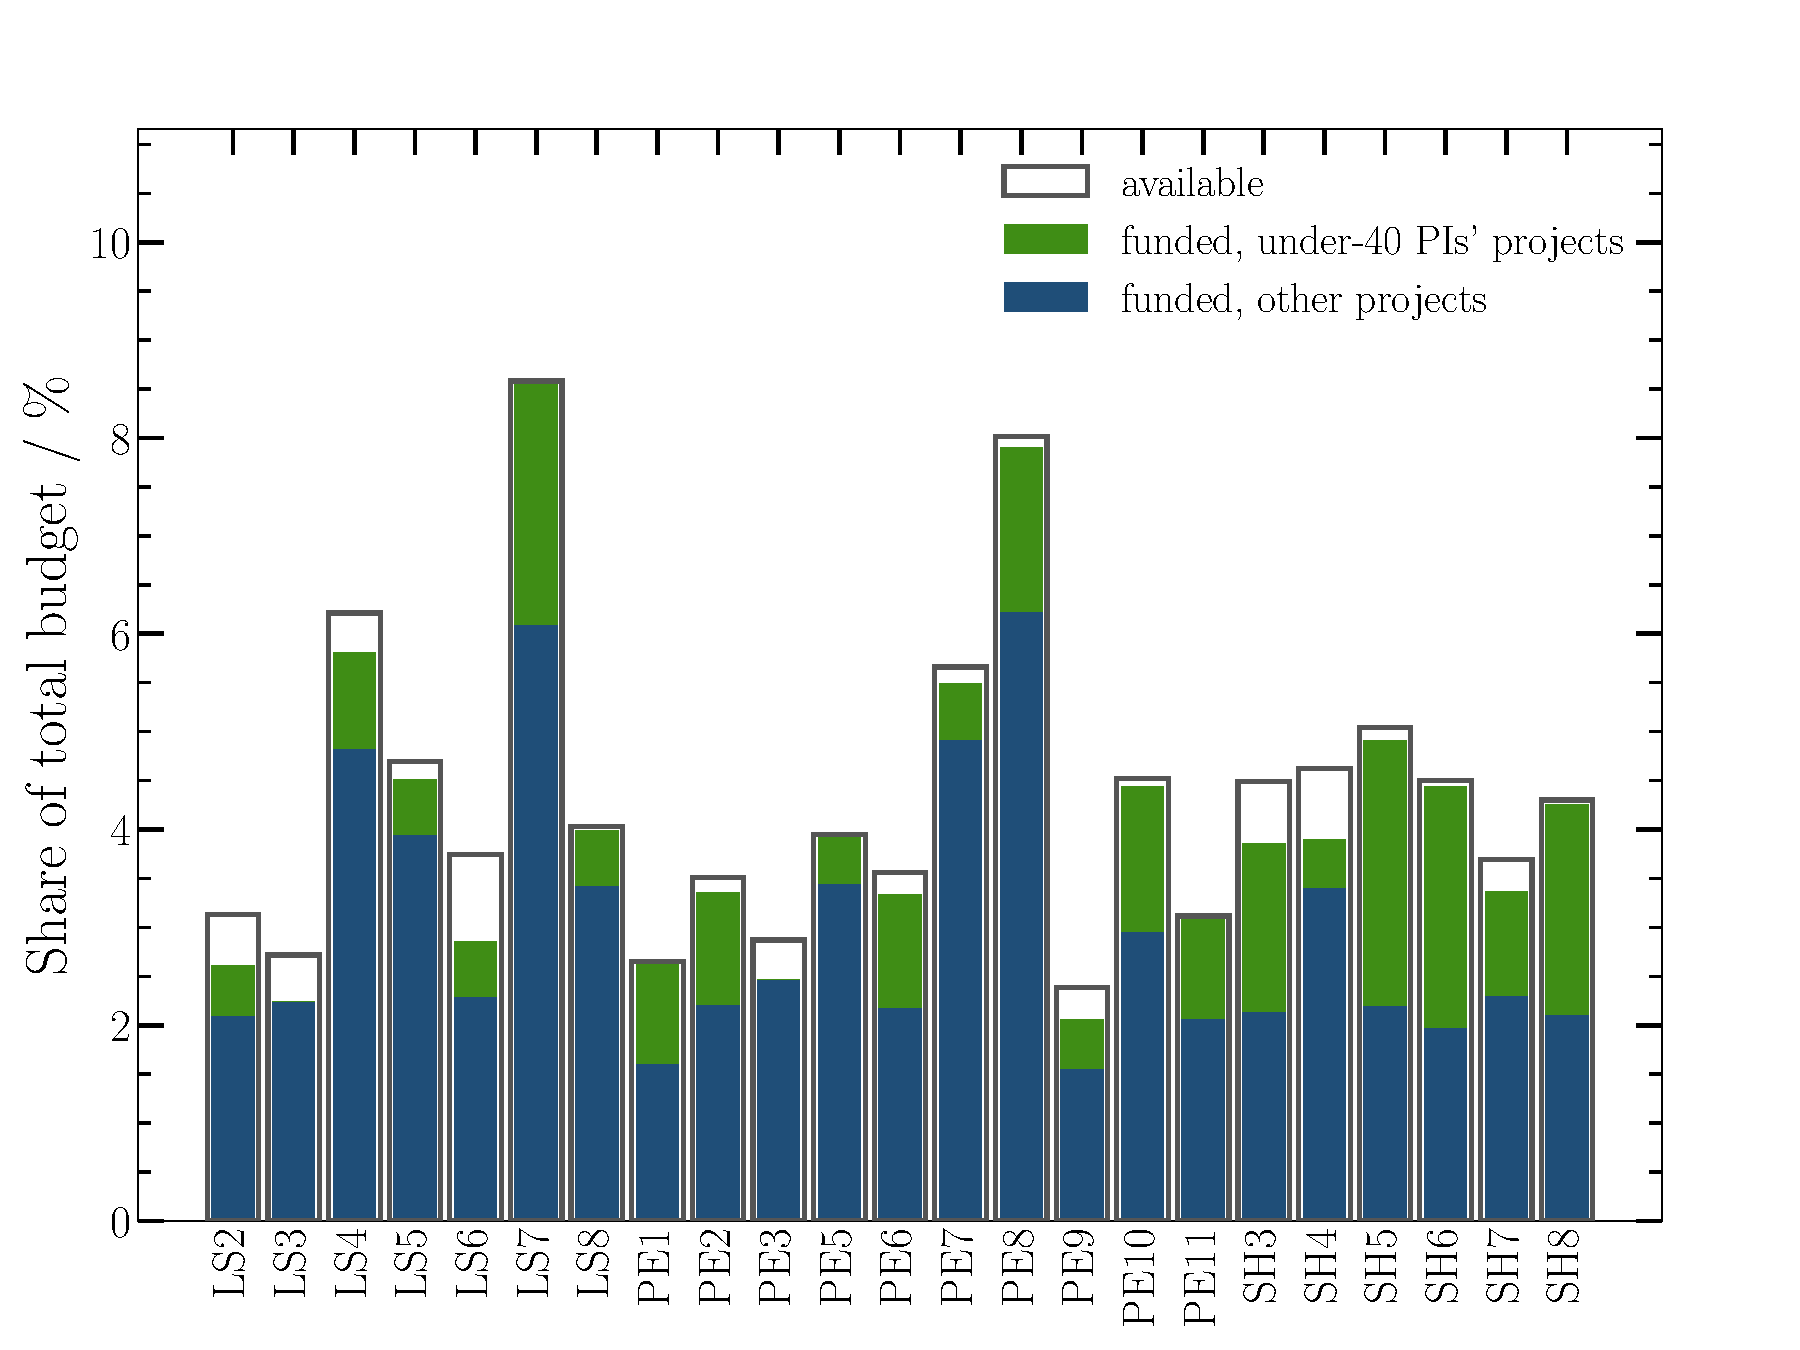
\includegraphics[width=0.85\textwidth]{../prin_out/figures/sector_budgets.pdf}
\caption{Per sector, in percent of the total budget: budget available (outline) and funded money, split into projects of under-40 PIs (green) and the others (blue). 18 of 28 sectors.}
\end{figure}

\subsection{Funding by institution}
\textbf{Purpose.} To show which institutions received the largest shares of the budget and how the budget is divided among institutions.

\textbf{Result.} 84 institutions have at least one funded unit. The largest share is that of CNR (7.2\%), followed by Sapienza (6.2\%) and Padova (4.6\%). The 10 best-funded institutions received 41.0\% of the budget and the 20 best-funded 61.0\%; after accounting for them, 59.0\% and 39.0\% of the budget are left.

\begin{figure}[H]
\centering
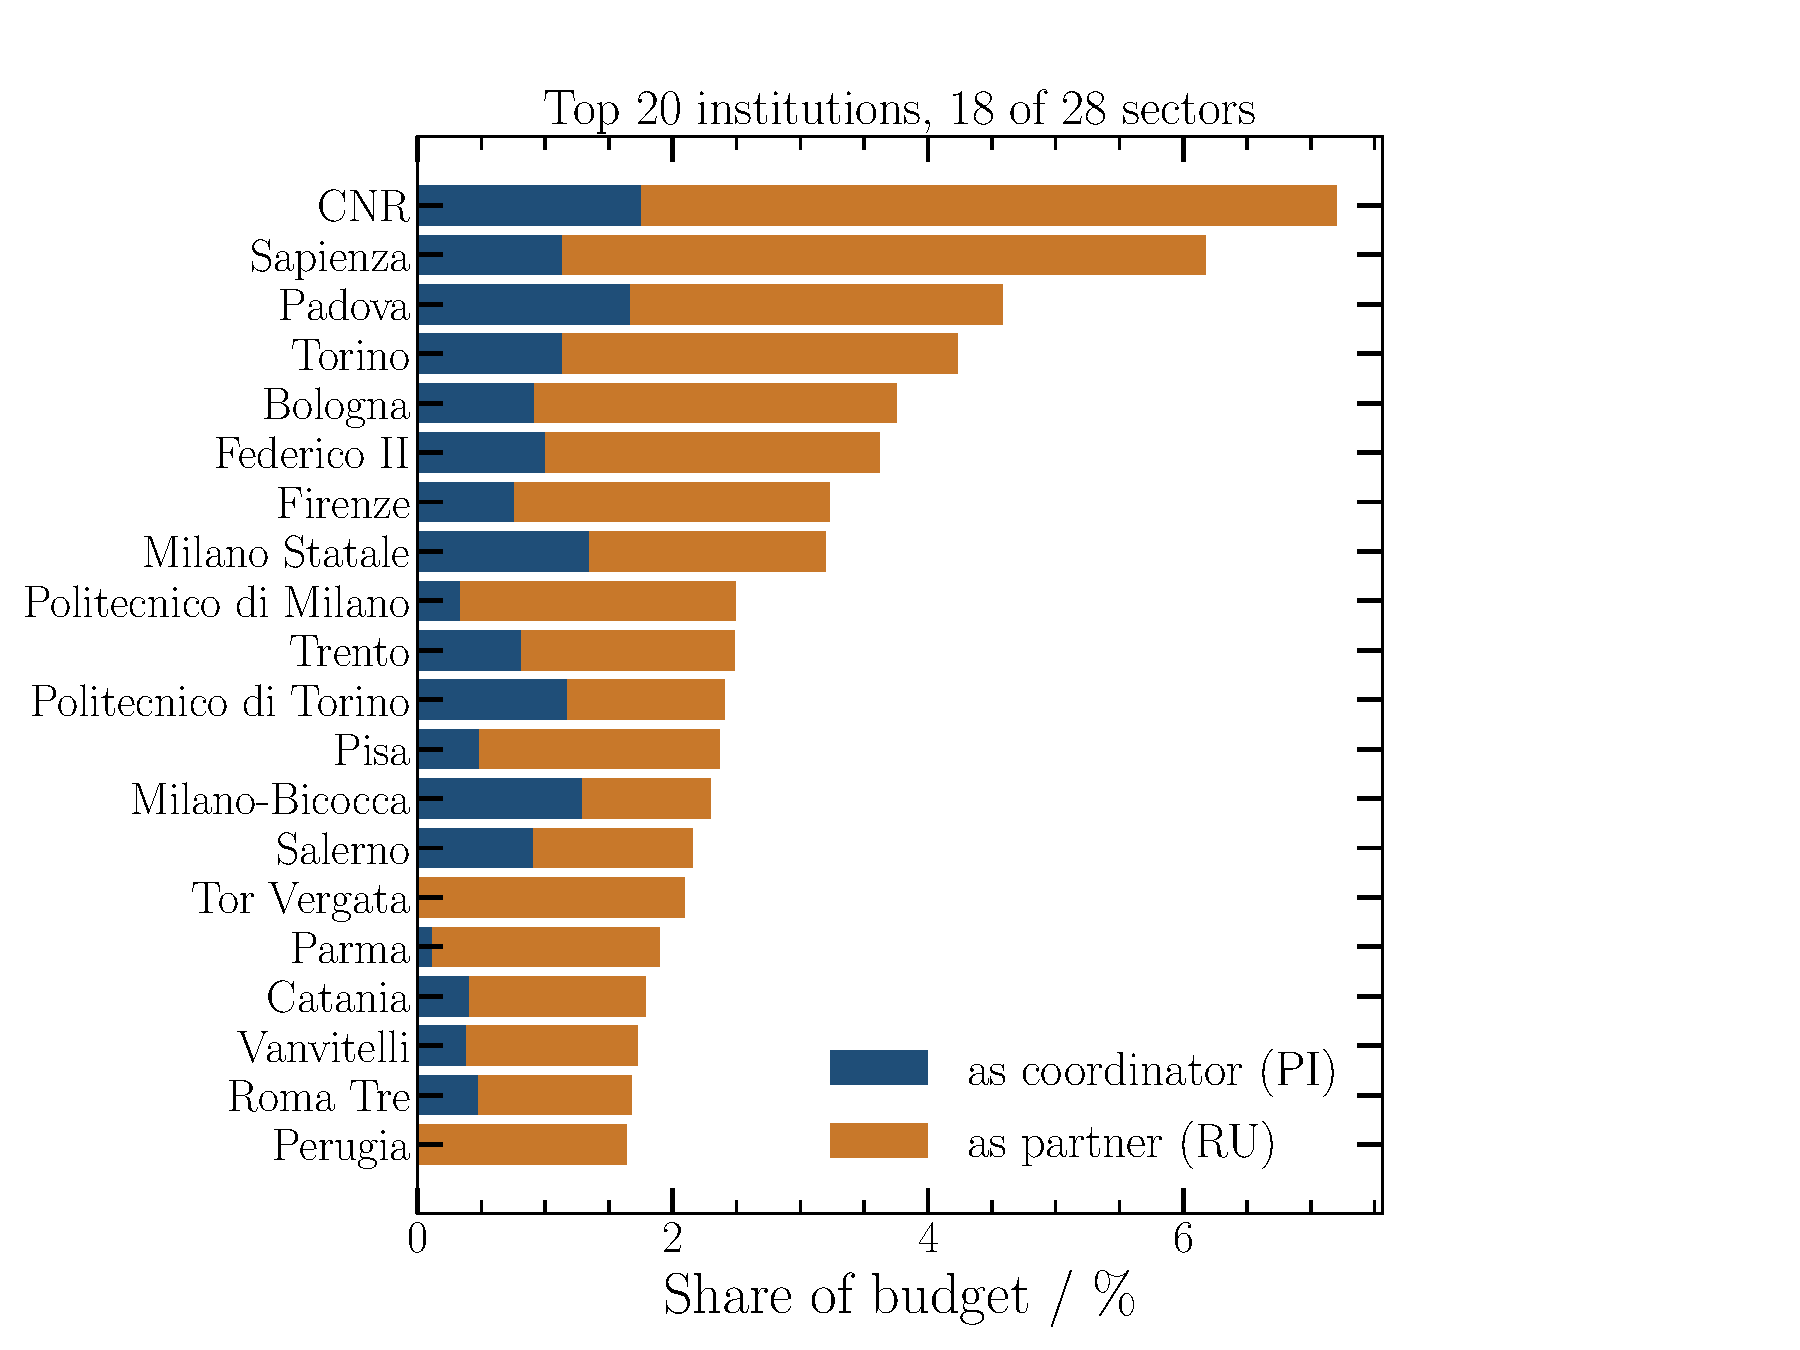
\includegraphics[width=0.7\textwidth]{../prin_out/figures/institutions_share.pdf}
\caption{Share of the total budget of the 20 best-funded institutions, as coordinator (PI) and as partner (RU).}
\end{figure}
\begin{figure}[H]
\centering
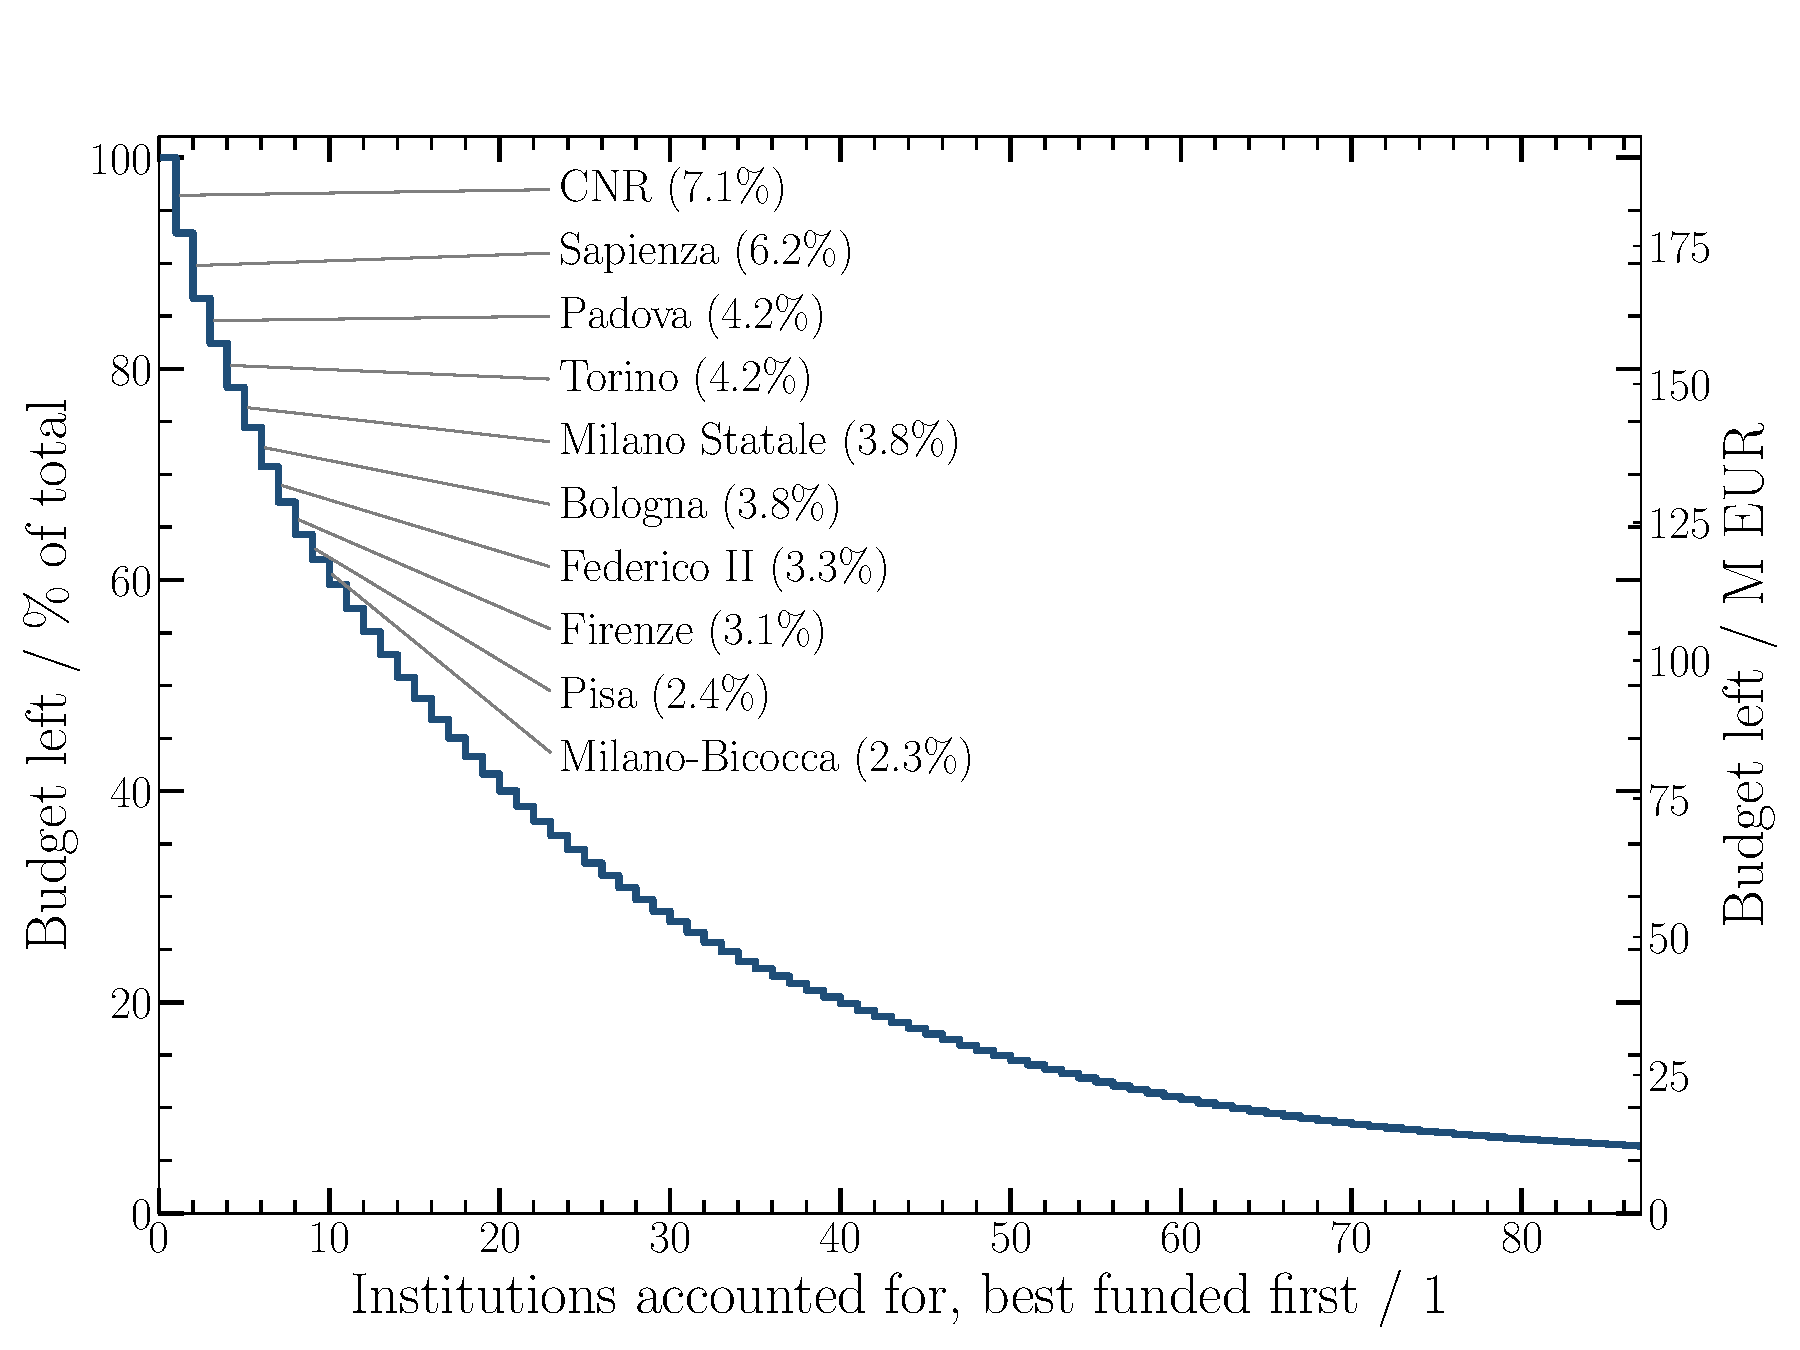
\includegraphics[width=0.8\textwidth]{../prin_out/figures/budget_by_institution.pdf}
\caption{Budget left, in percent of the total, as the institutions are accounted for from the best funded to the least funded; the ten largest steps are named.}
\end{figure}

\subsection{Institution types}
\textbf{Purpose.} To show how the budget is divided among types of institution (public and private universities, telematic universities, advanced schools, research bodies).

\textbf{Result.} Public universities received 76.9\% of the budget, national research bodies 9.4\%, private universities 3.9\%, advanced schools 2.7\%, telematic universities 1.3\%. The table gives the number of institutions and the shares by role.

\begin{table}[H]
\centering
\begin{tabular}{lrrrrr}
\toprule
Type & Institutions & Projects & Share (\%) & as PI (\%) & as RU (\%) \\
\midrule
Public univ. & 58 & 144 & 76.88 & 20.11 & 56.77 \\
Private univ. & 8 & 28 & 3.87 & 0.73 & 3.14 \\
Telematic univ. & 4 & 12 & 1.32 & 0.00 & 1.32 \\
Advanced schools & 7 & 15 & 2.71 & 1.34 & 1.37 \\
Research bodies & 2 & 4 & 0.50 & 0.00 & 0.50 \\
National bodies & 4 & 58 & 9.36 & 2.07 & 7.29 \\
AFAM & 1 & 1 & 0.10 & 0.00 & 0.10 \\
\bottomrule
\end{tabular}
\end{table}
\begin{figure}[H]
\centering
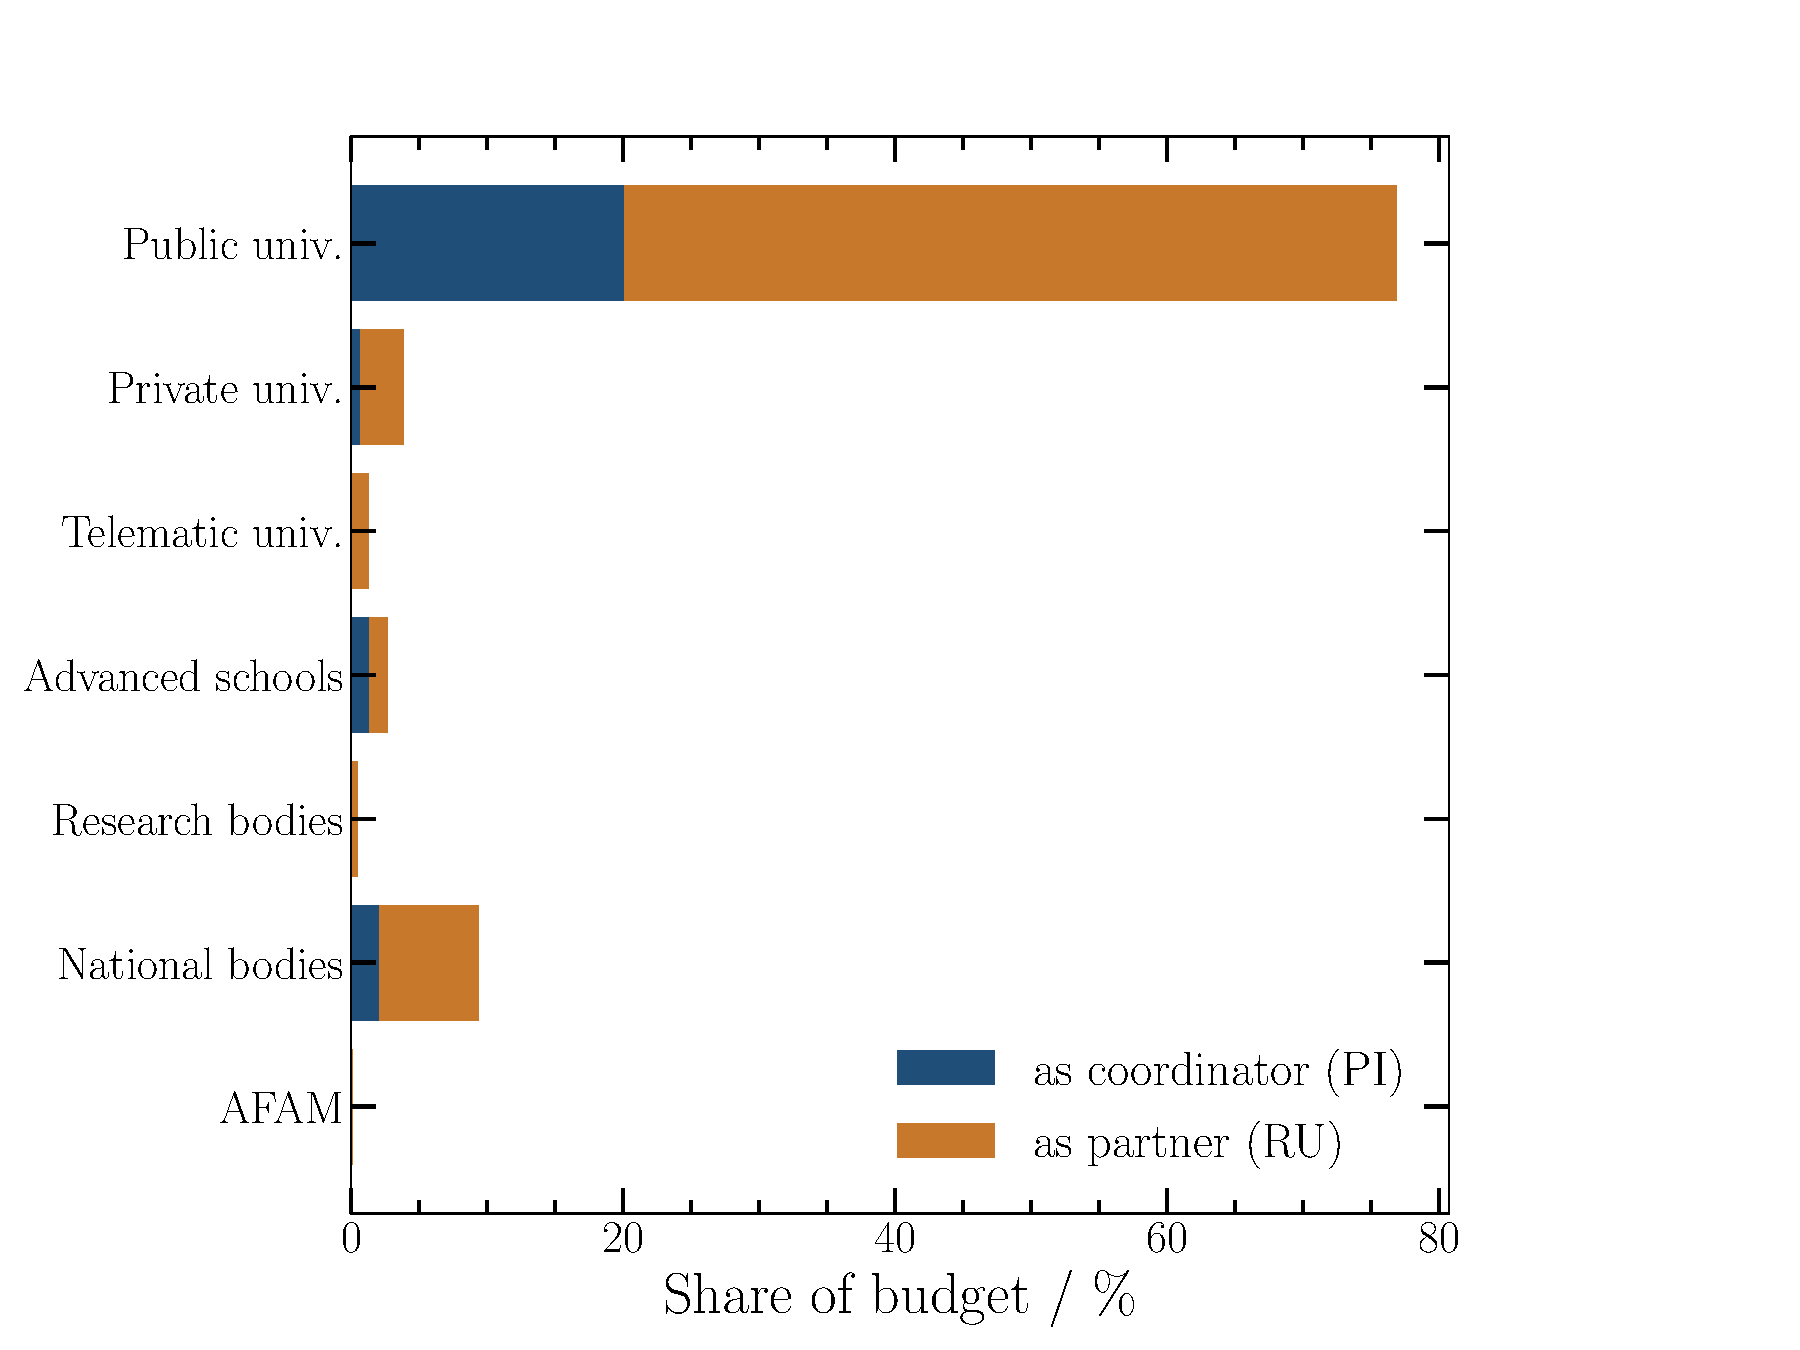
\includegraphics[width=0.7\textwidth]{../prin_out/figures/institution_types.pdf}
\caption{Share of the total budget by institution type, as coordinator (PI) and as partner (RU).}
\end{figure}

\subsection{MUR contribution per unit}
\textbf{Purpose.} To show the distribution of the money assigned to a single unit, for coordinating and for partner units.

\textbf{Result.} The 144 coordinating units received a median of 258~k~EUR (quartiles 222 and 303; range 150 to 618~k~EUR). The 582 partner units received a median of 193~k~EUR (quartiles 167 and 222; range 56 to 489~k~EUR).

\begin{figure}[H]
\centering
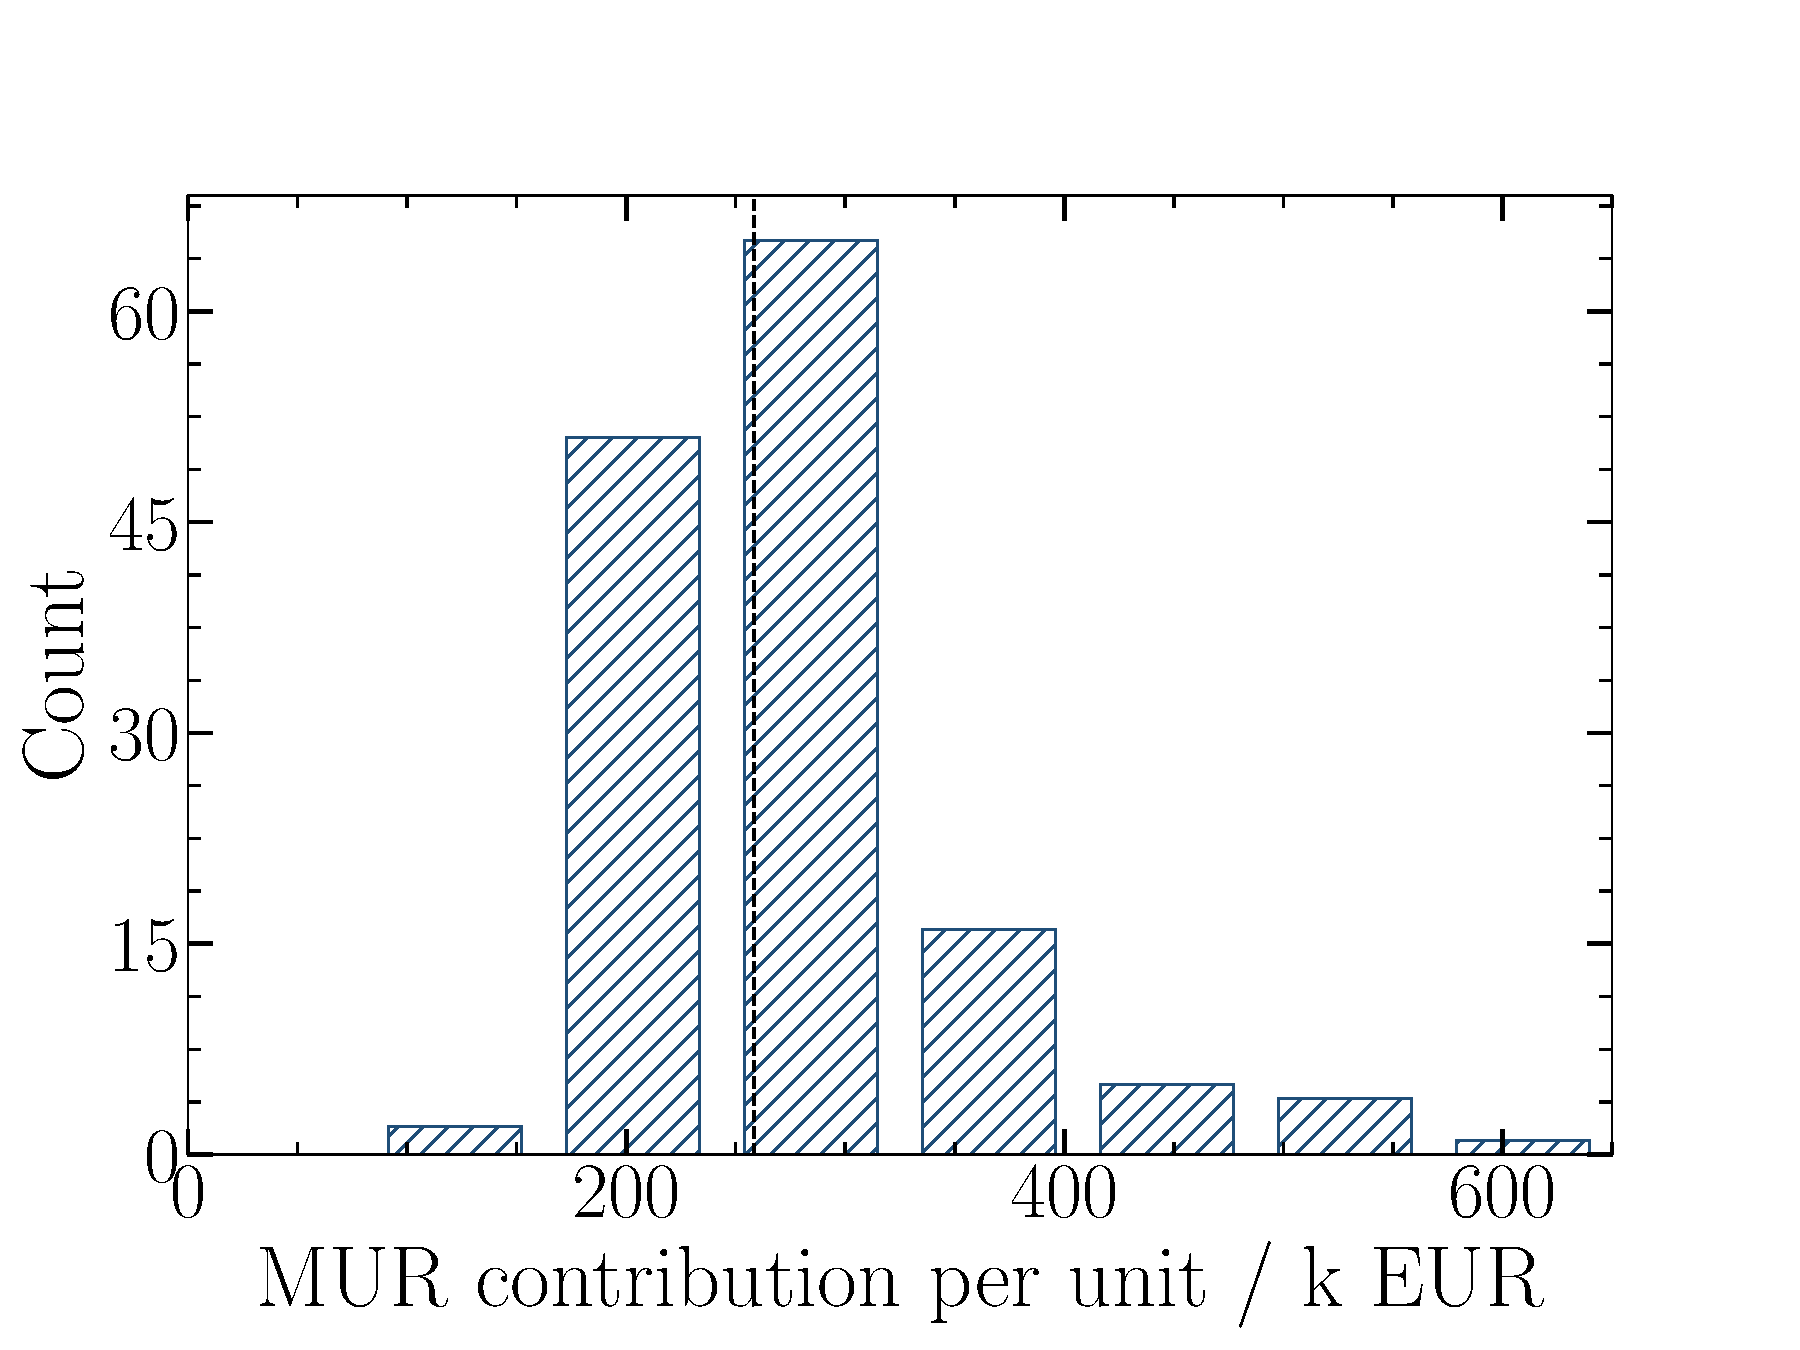
\includegraphics[width=0.6\textwidth]{../prin_out/figures/money_per_unit_coordinating.pdf}
\caption{Histogram of the MUR contribution of the coordinating units; the dashed line is the median.}
\end{figure}
\begin{figure}[H]
\centering
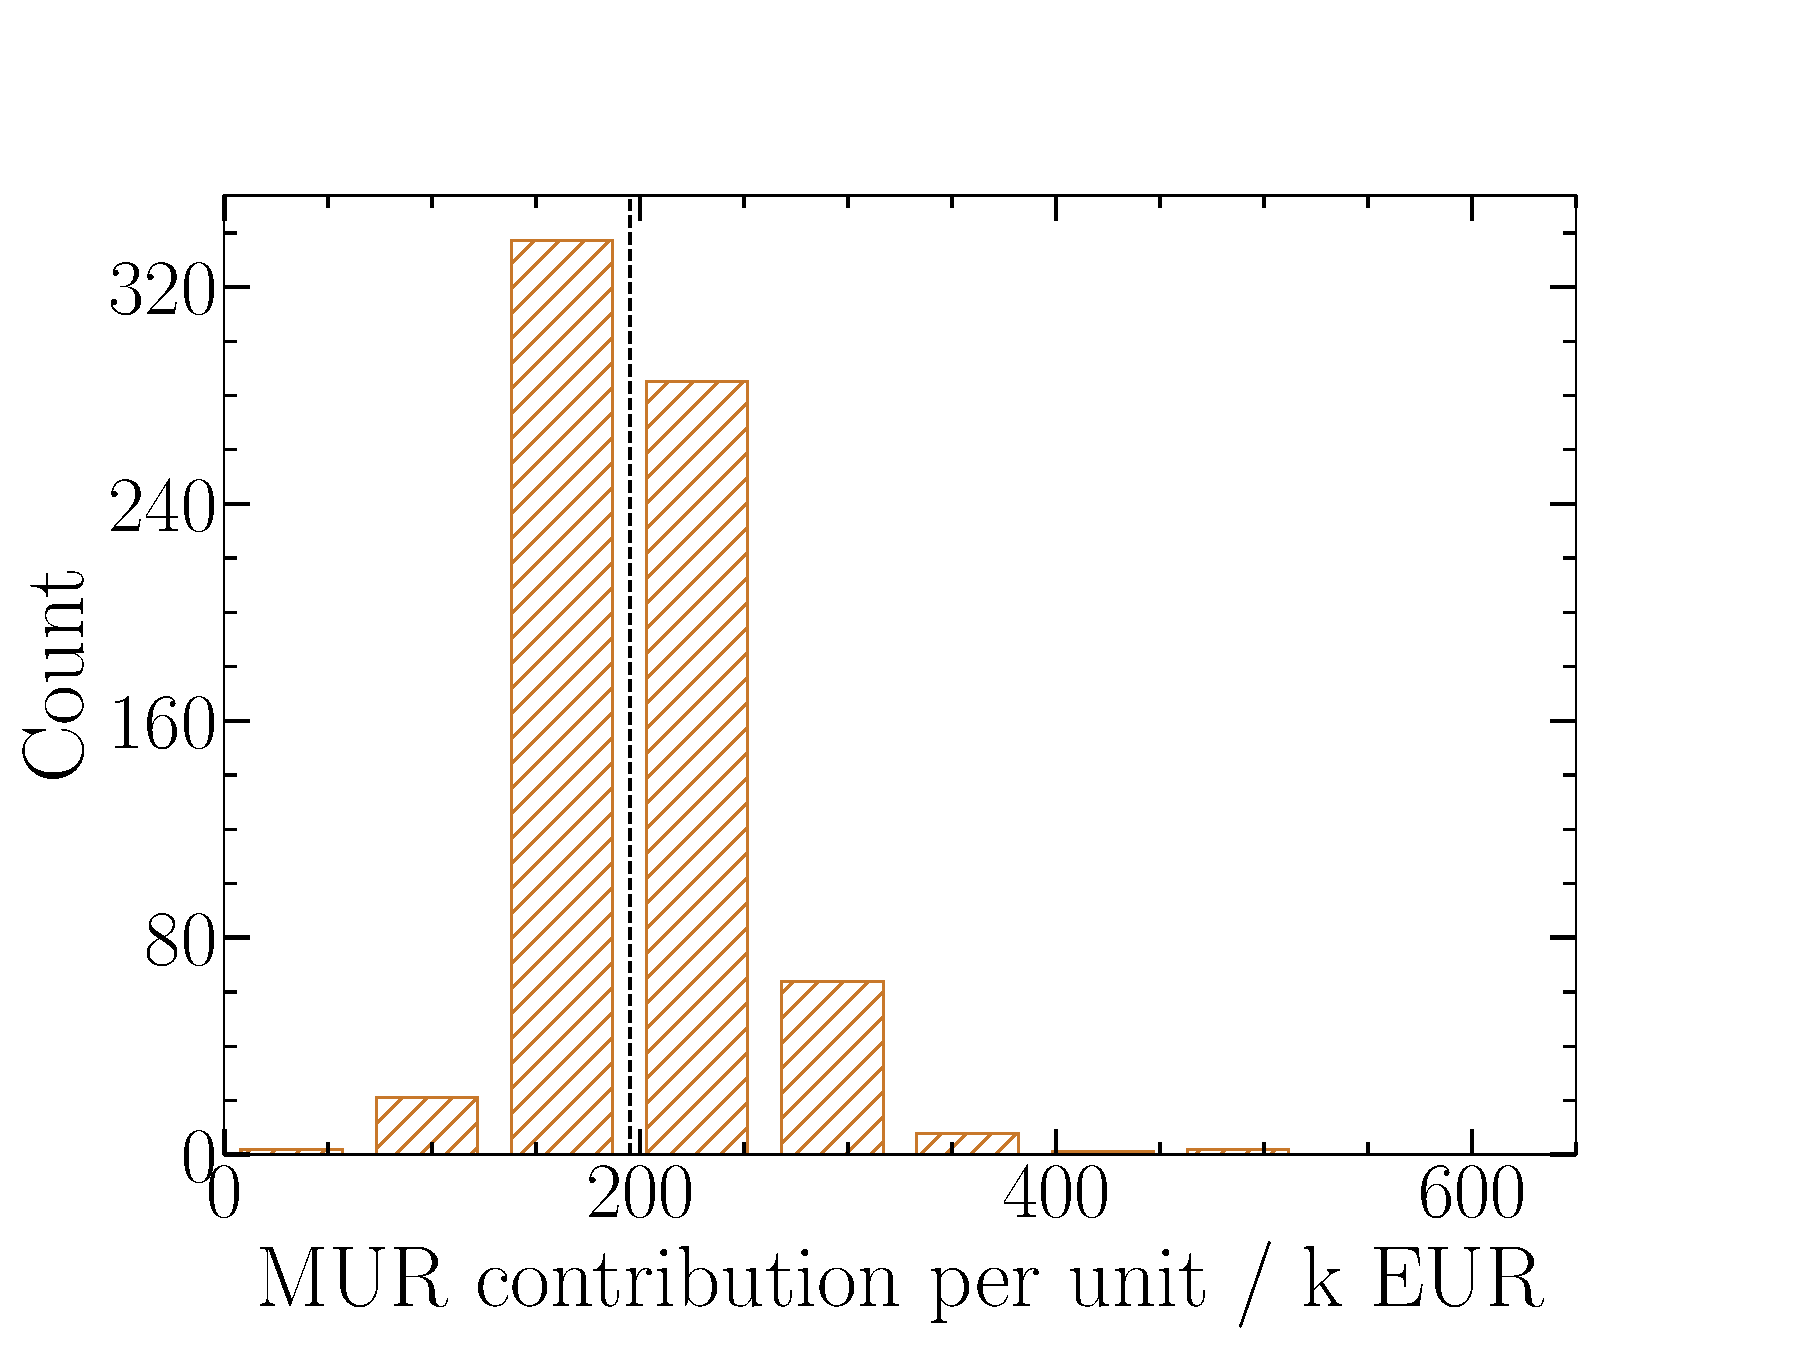
\includegraphics[width=0.6\textwidth]{../prin_out/figures/money_per_unit_partner.pdf}
\caption{Histogram of the MUR contribution of the partner units; the dashed line is the median.}
\end{figure}

\subsection{Geography}
\textbf{Purpose.} To show where the money went: by region, by city, and, per region and macro-area, which part of the funding came from units coordinating projects and which from partner units.

\textbf{Result.} The regions with the largest shares are Lombardia (14.4\%), Lazio (12.9\%) and Campania (8.9\%). National research bodies (CNR, INAF, INFN, INGV), which have no region, received 9.4\%. No funded unit is in Valle d'Aosta. The 53 cities with a funded unit include Roma (11.8\%), Milano (10.3\%), Torino (6.9\%), Napoli (4.9\%) and Padova (4.6\%) as the five largest. The share of the money received by units coordinating projects is, by macro-area: North 30\%; Centre 21\%; South and Islands 24\%. Liguria, Molise, Basilicata and Calabria have no coordinating unit among their funded units. The table of regions is in Appendix C.

\begin{figure}[H]
\centering
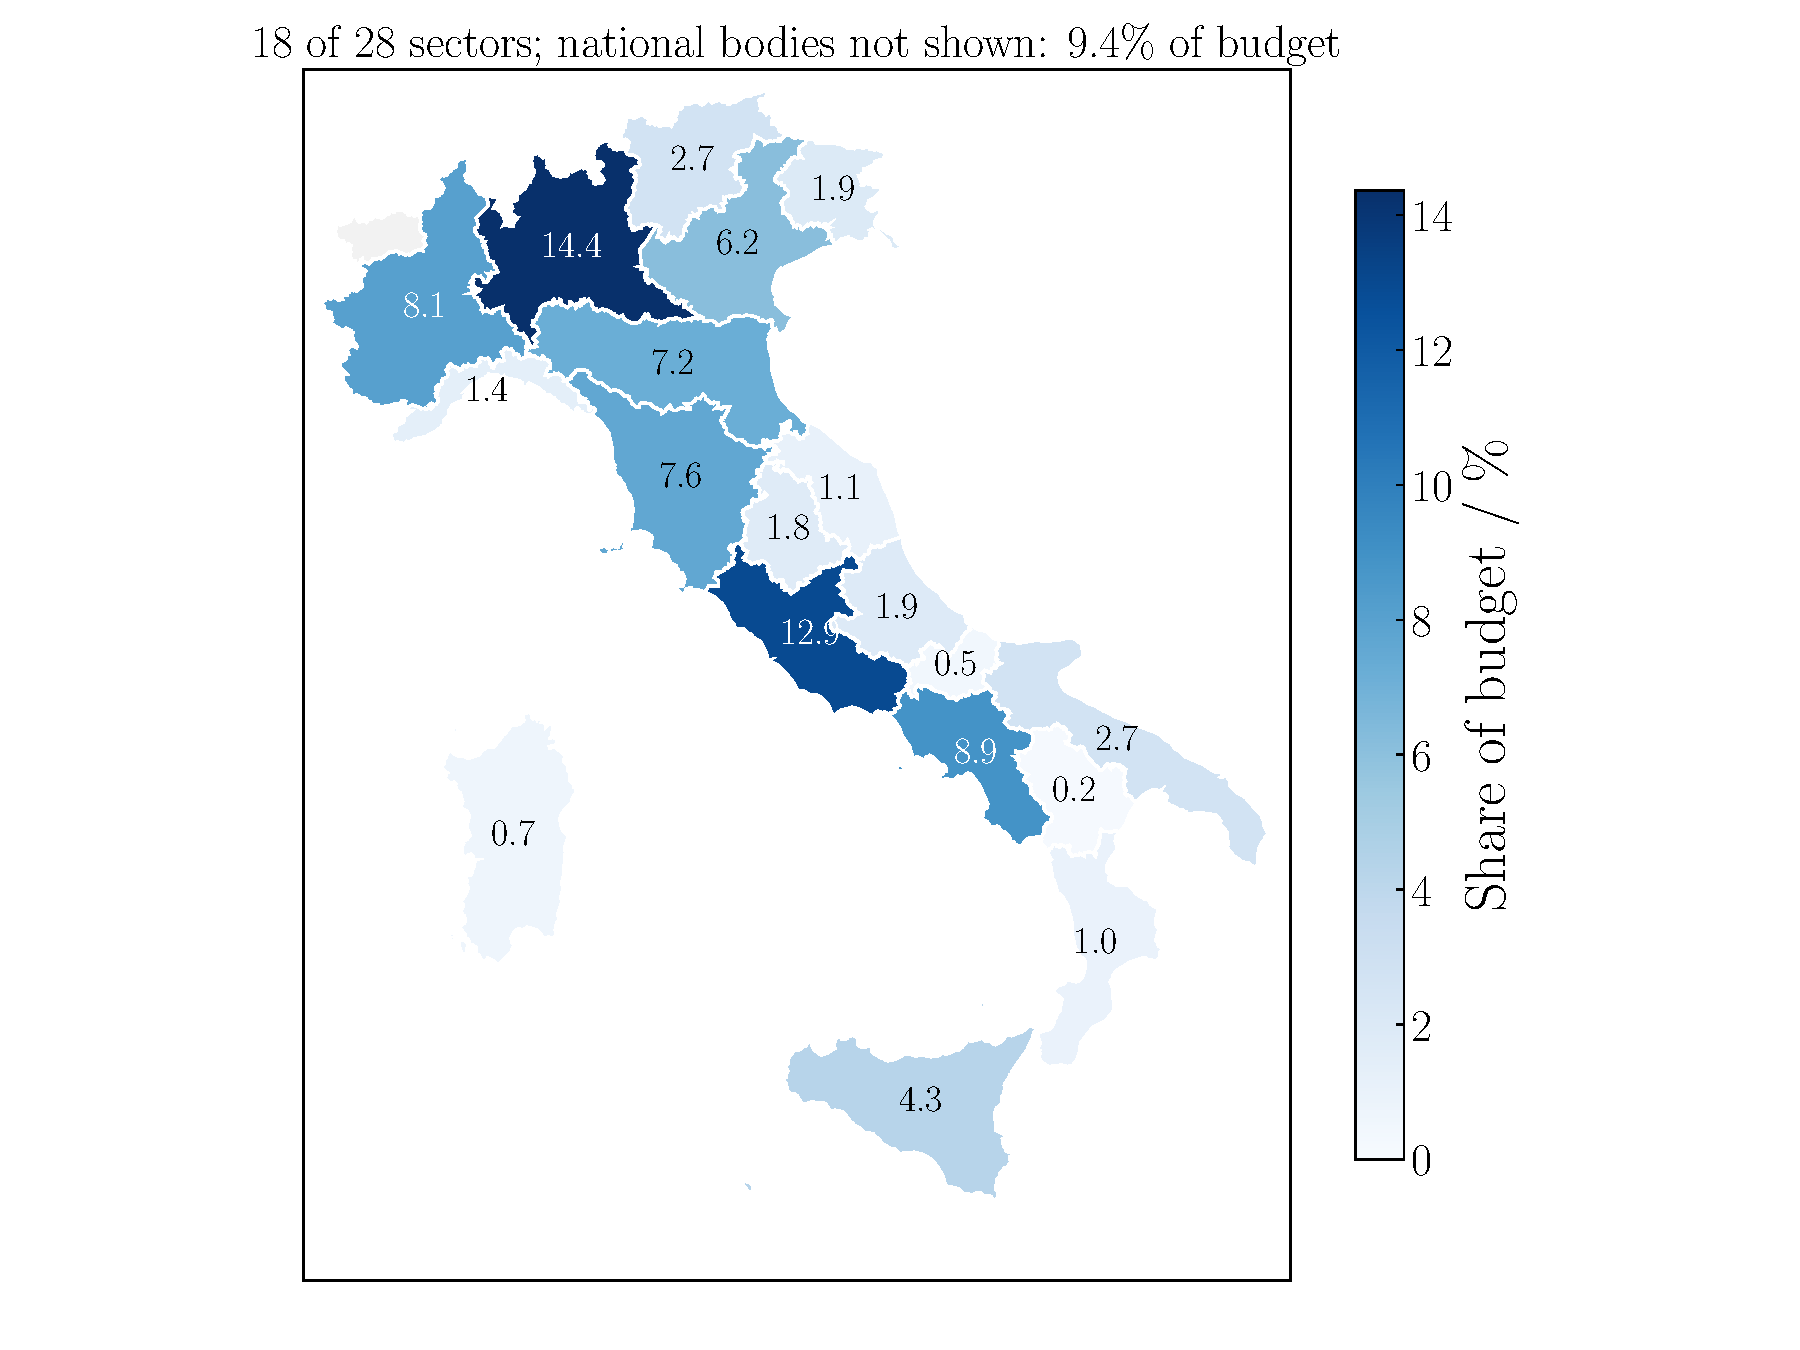
\includegraphics[width=0.7\textwidth]{../prin_out/figures/map_regions_share.pdf}
\caption{Share of the total budget by region; national research bodies are not shown.}
\end{figure}
\begin{figure}[H]
\centering
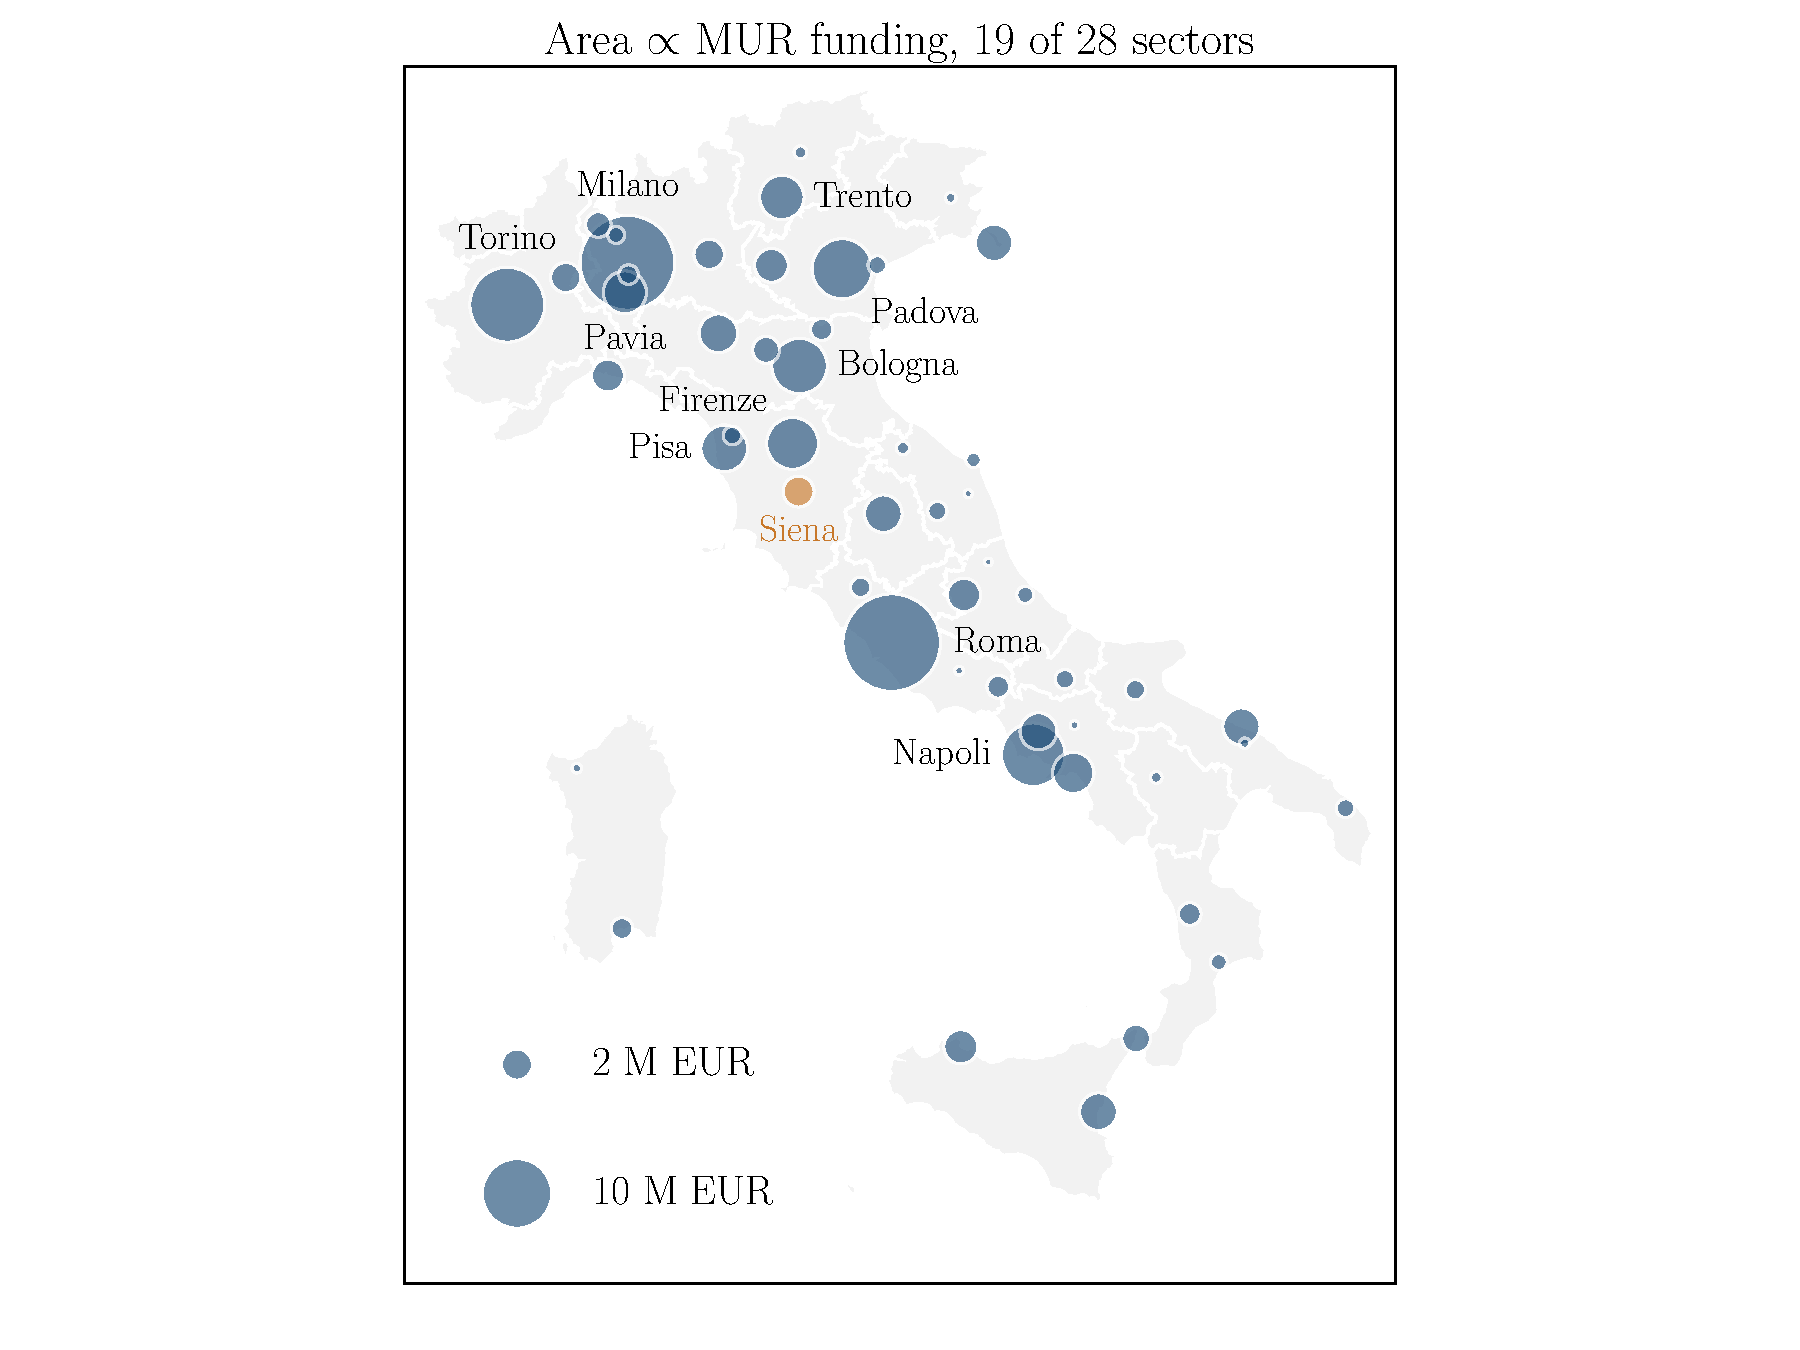
\includegraphics[width=0.7\textwidth]{../prin_out/figures/map_cities_funding.pdf}
\caption{MUR funding by city (circle area proportional to the money).}
\end{figure}
\begin{figure}[H]
\centering
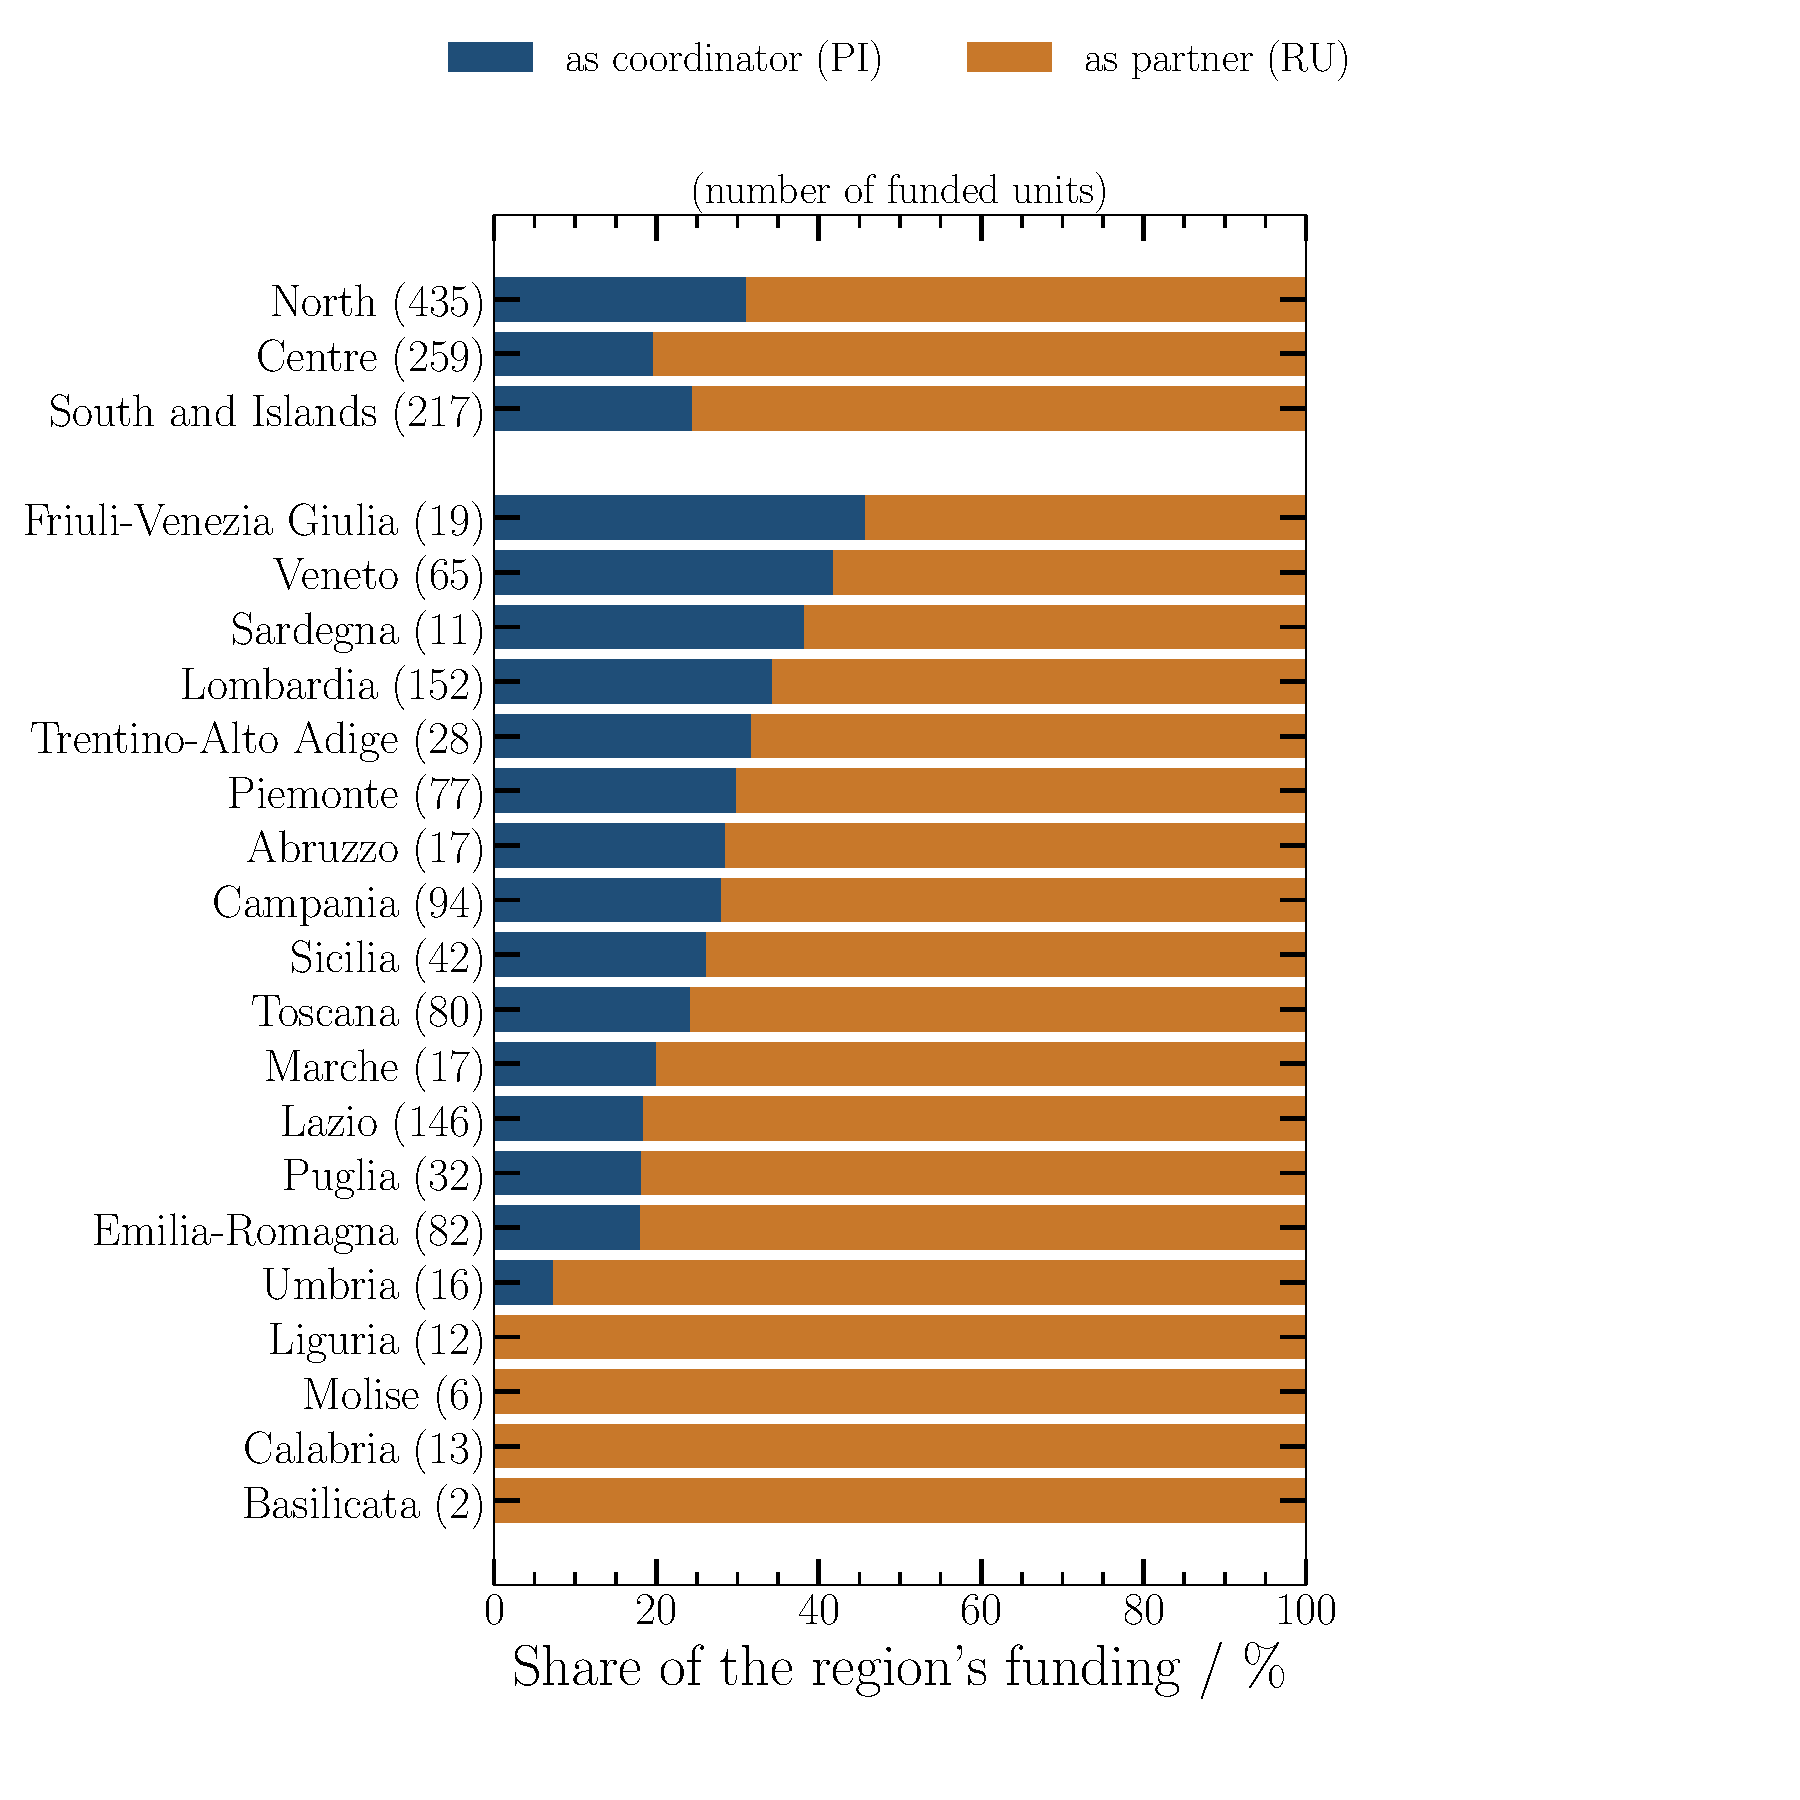
\includegraphics[width=0.75\textwidth]{../prin_out/figures/regions_roles.pdf}
\caption{Share of each macro-area's and region's funding received as coordinating (PI) and as partner (RU) units; in brackets, the number of funded units.}
\end{figure}

\subsection{Collaboration between cities}
\textbf{Purpose.} To show which cities share funded projects, counting the national research bodies as one node.

\textbf{Result.} 511 pairs of nodes share at least one funded project and 28 share eight or more. The pairs sharing the most projects are national bodies--Roma (28), Milano--Roma (27), national bodies--Torino (25), Milano--national bodies (24) and Milano--Torino (23).

\begin{figure}[H]
\centering
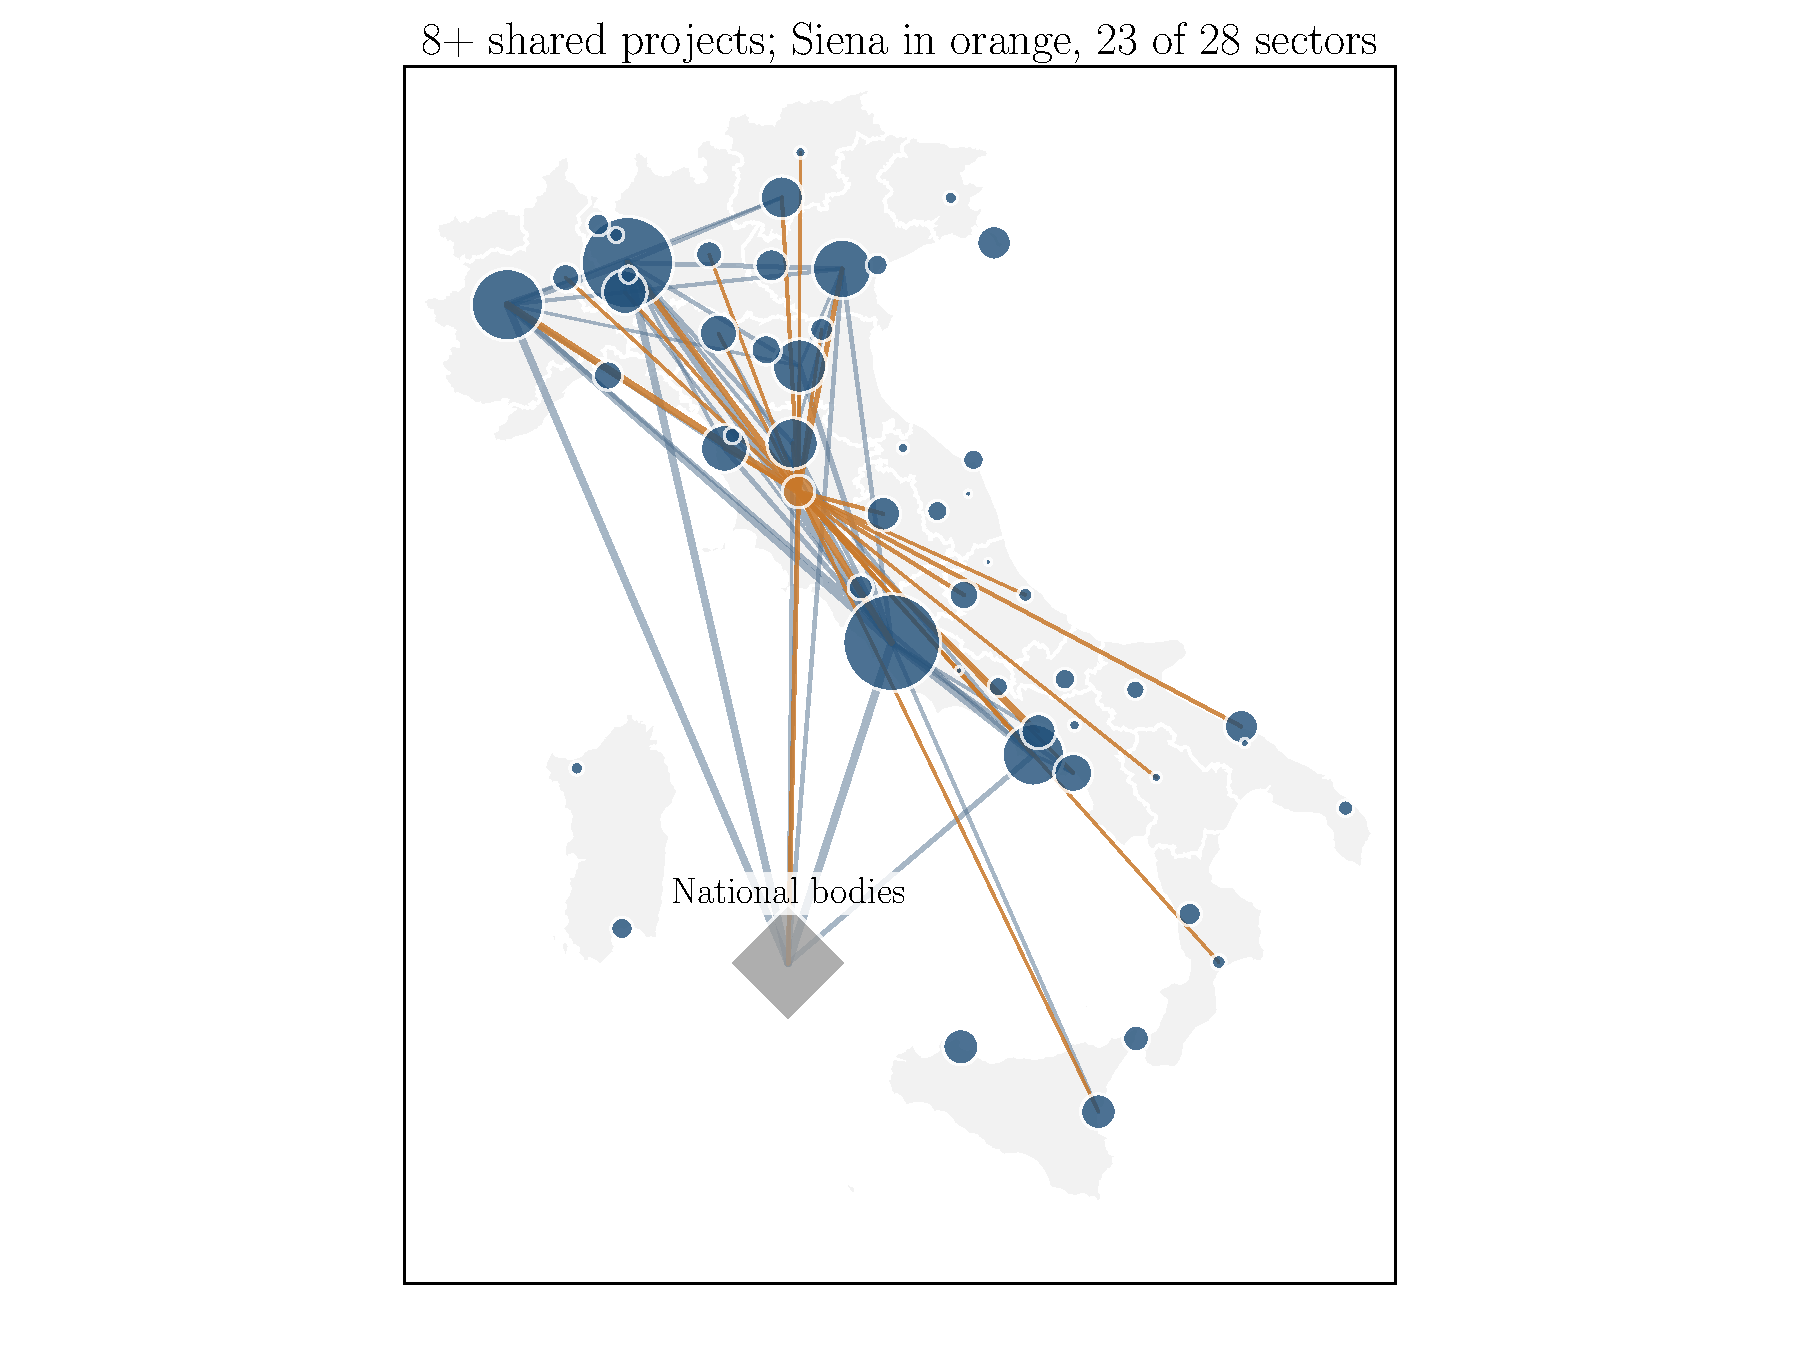
\includegraphics[width=0.75\textwidth]{../prin_out/figures/collaboration_map.pdf}
\caption{Pairs of cities sharing at least 8 funded projects (line width proportional to the number); circle area proportional to the money; the diamond is the national research bodies. 18 of 28 sectors.}
\end{figure}

\subsection{Breadth across sectors}
\textbf{Purpose.} To show in how many sectors each institution has funded units, against the share of the budget it received.

\textbf{Result.} The number of sectors with at least one funded unit has median 3 across the 84 institutions; 19 institutions have funded units in one sector only. The maximum, 16 sectors, is reached by Padova. The Spearman correlation between the number of sectors and the money received is 0.94 (p = 4e-39).

\begin{figure}[H]
\centering
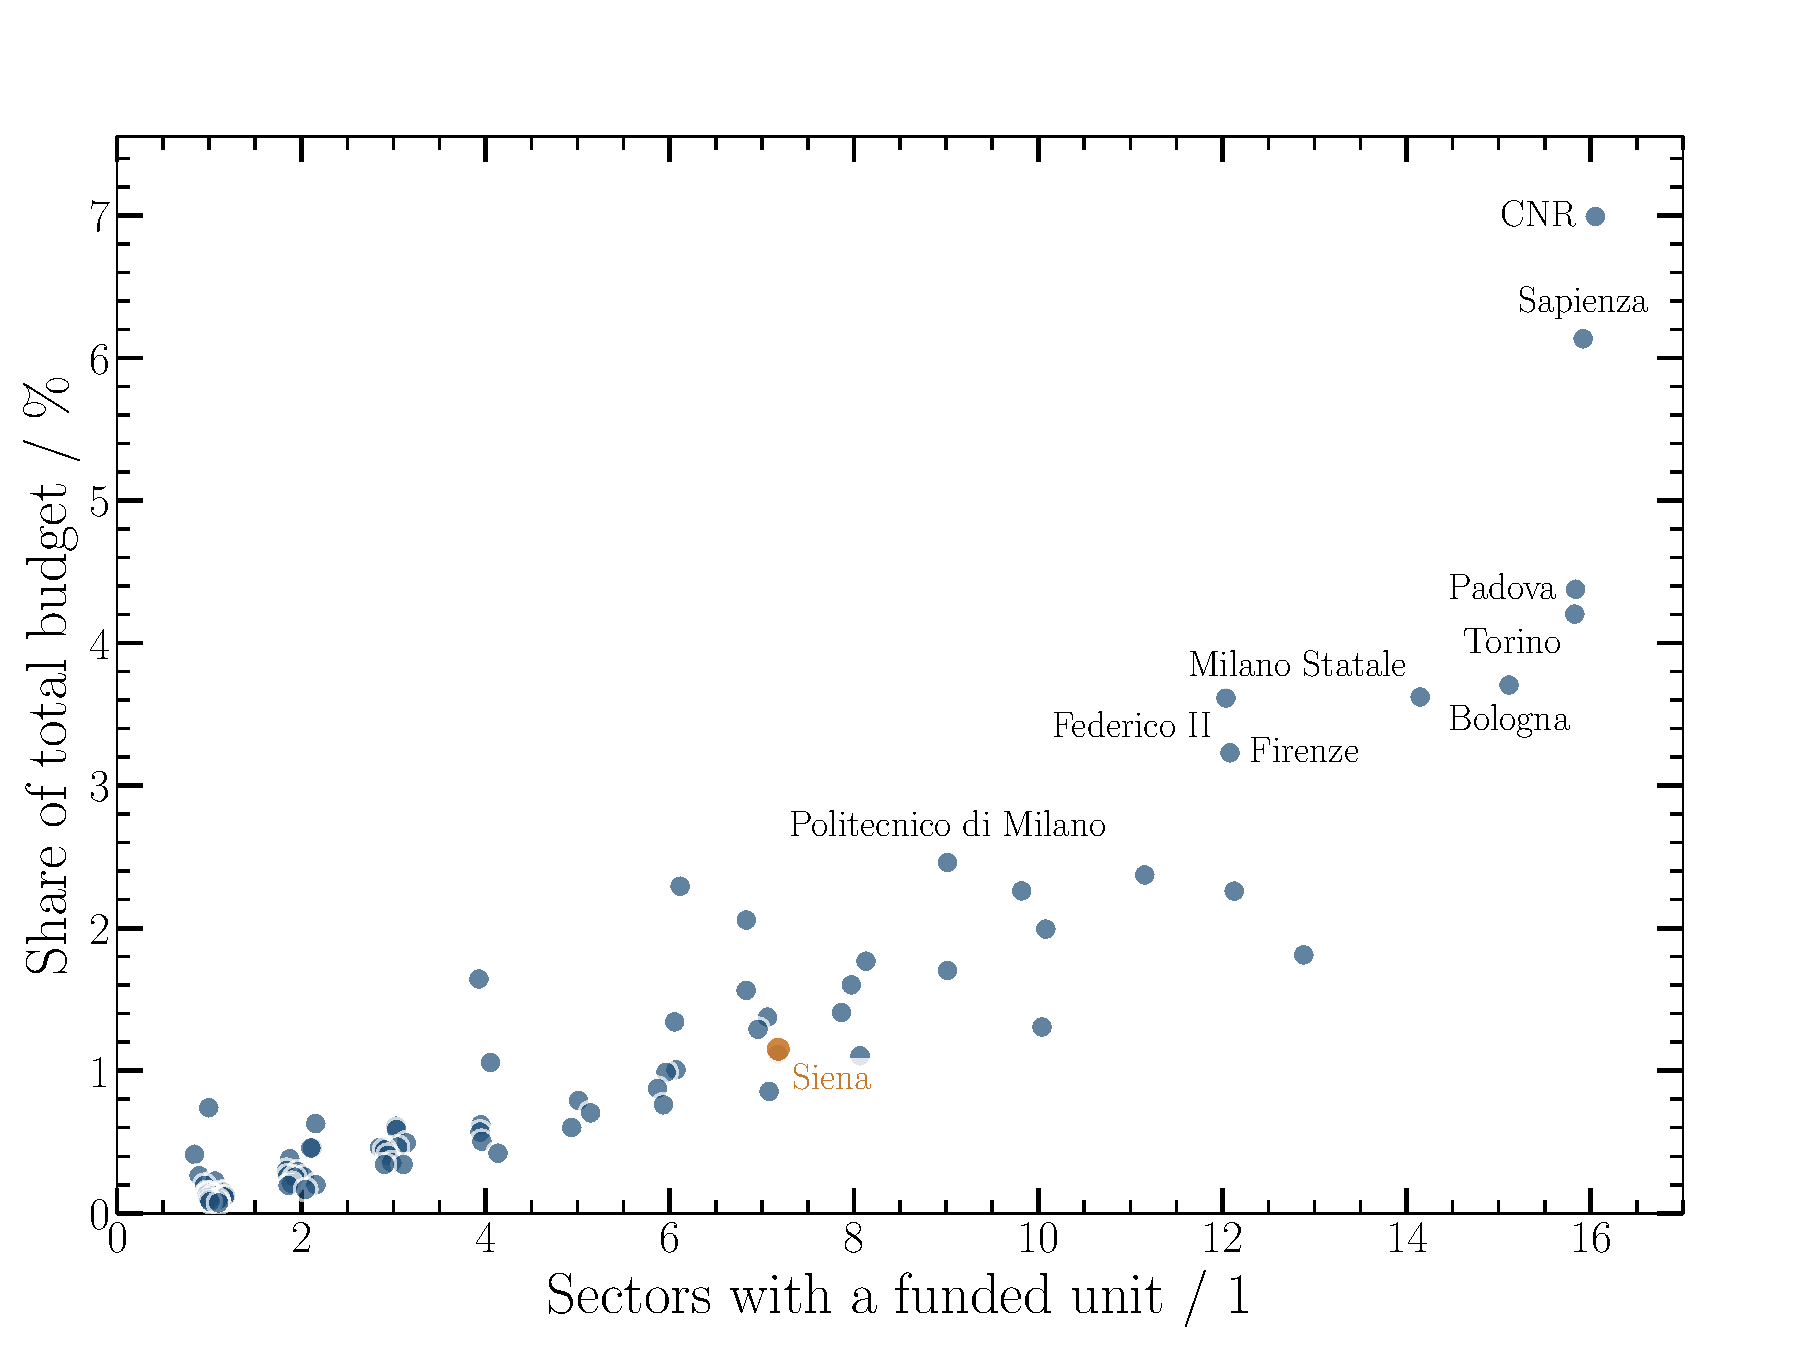
\includegraphics[width=0.75\textwidth]{../prin_out/figures/institution_breadth.pdf}
\caption{Share of the total budget of each institution against the number of sectors with a funded unit (horizontal jitter added).}
\end{figure}

\subsection{Gender of the unit leaders}
\textbf{Purpose.} To show the share of women among the leaders of the funded units, with the uncertainty due to the small numbers, by macro-area (PE, LS, SH).

\textbf{Result.} Among the 144 funded PIs, 33\% are women (95\% interval 26--41); among the 582 leaders of funded partner units, 37\% (33--41). The first given name was found in the name table for all 726 leaders considered. The table gives the shares by macro-area.

\begin{table}[H]
\centering
\begin{tabular}{llrrr}
\toprule
Group & Area & Leaders & Women (\%) & 95\% interval \\
\midrule
PI, funded & PE & 74 & 28 & 19--40 \\
PI, funded & LS & 38 & 37 & 23--53 \\
PI, funded & SH & 32 & 41 & 26--58 \\
PI, funded & All & 144 & 33 & 26--41 \\
Partner-unit leaders, funded & PE & 305 & 25 & 21--30 \\
Partner-unit leaders, funded & LS & 153 & 50 & 42--58 \\
Partner-unit leaders, funded & SH & 124 & 48 & 39--56 \\
Partner-unit leaders, funded & All & 582 & 37 & 33--41 \\
\bottomrule
\end{tabular}
\end{table}
\begin{figure}[H]
\centering
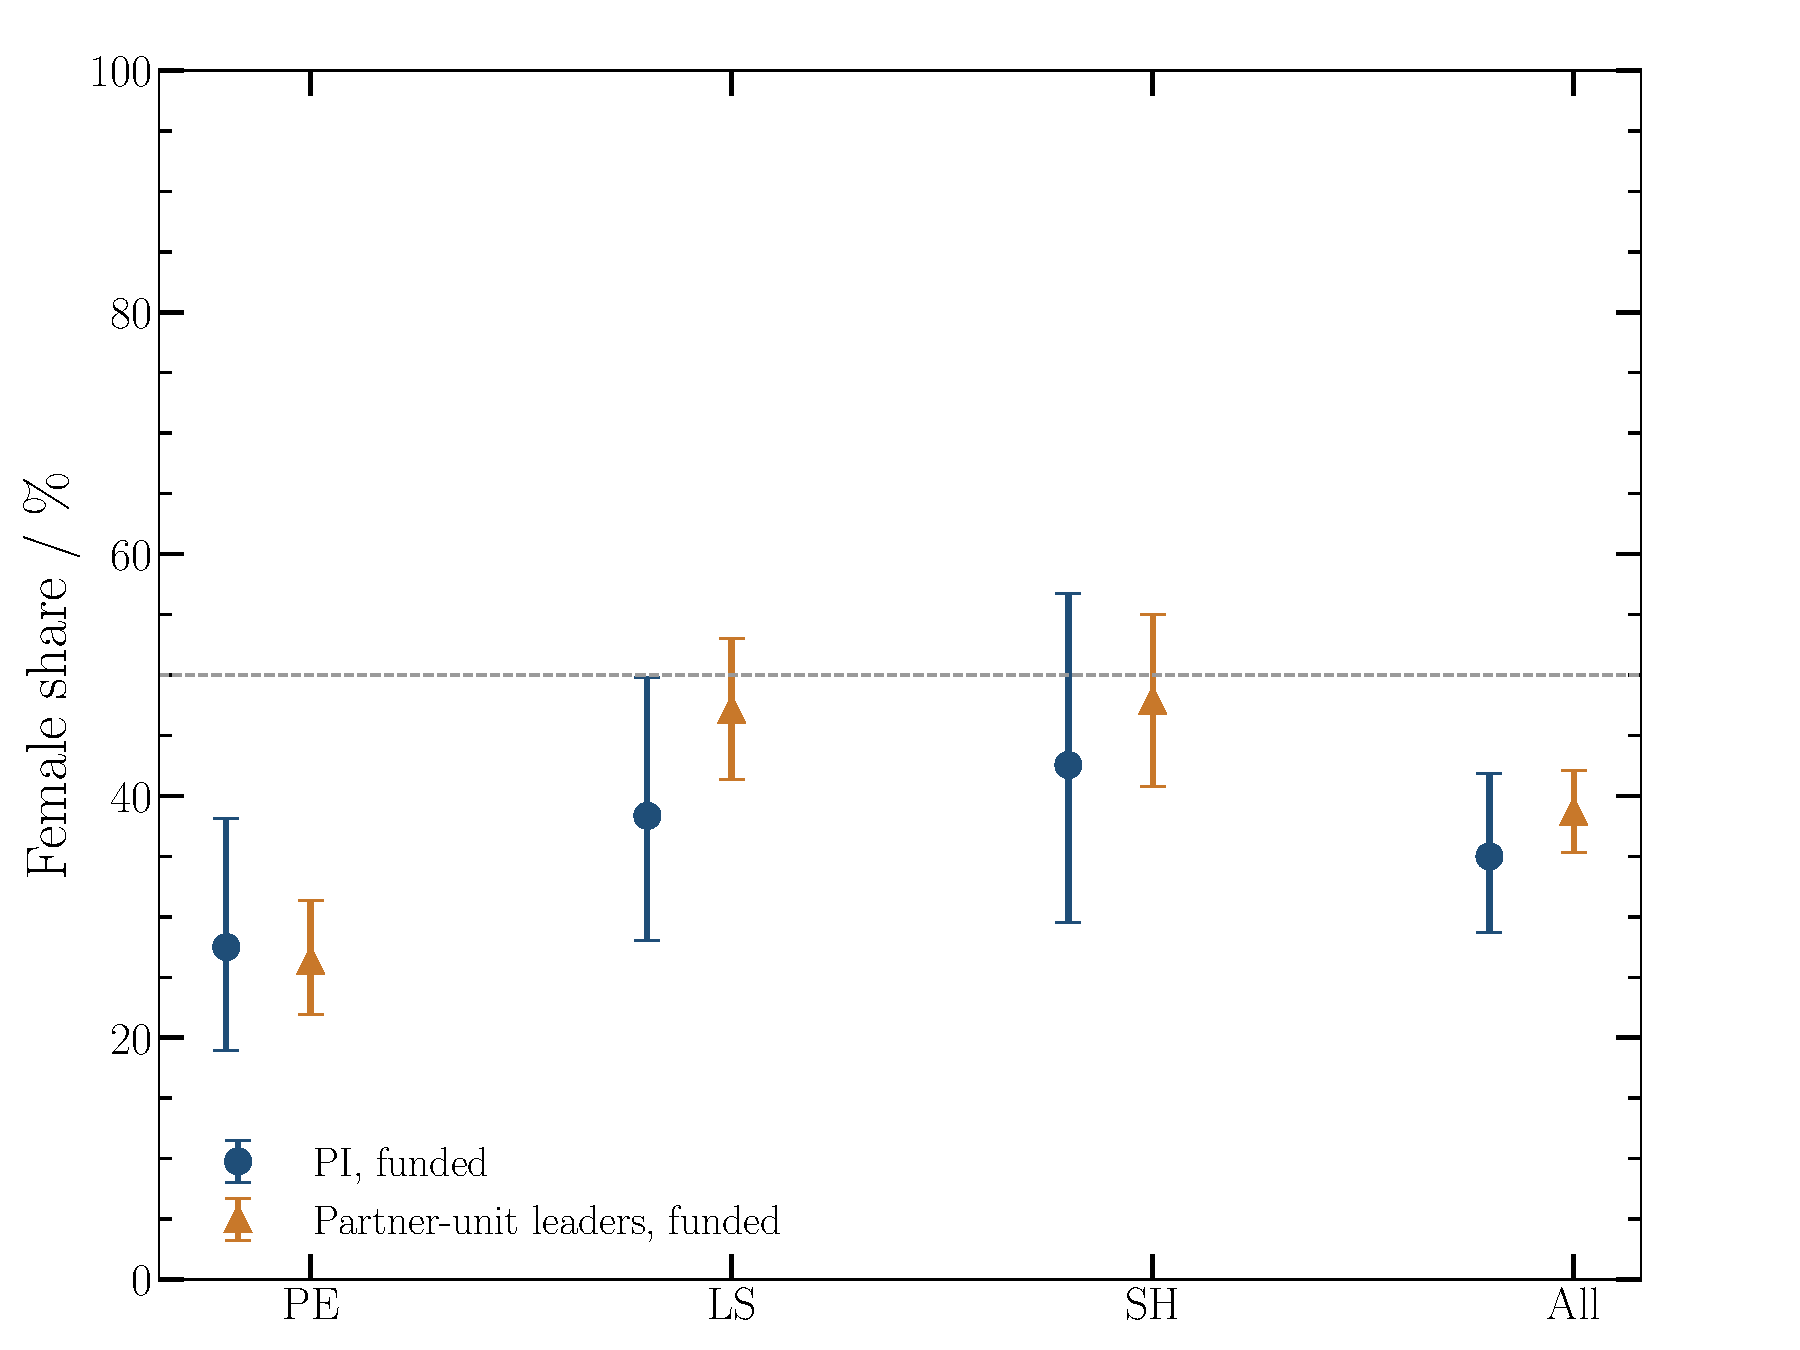
\includegraphics[width=0.7\textwidth]{../prin_out/figures/gender.pdf}
\caption{Share of women among the leaders of the funded units, with Wilson 95\% intervals; the dashed line marks 50\%.}
\end{figure}

\subsection{Budget, population and university staff by region}
\textbf{Purpose.} To compare the share of the budget of each region with its share of the resident population and of the professors and researchers of its universities.

\textbf{Result.} Across the 19 regions with funded units, the share of the budget has Pearson correlation 0.91 and Spearman correlation 0.83 with the share of the resident population, and 0.96 and 0.88 with the share of professors and researchers (national research bodies excluded; Valle d'Aosta has no funded unit and is left out). The table gives the shares and, in the last two columns, the share of the budget divided by the share of the population and of the staff.

\begin{table}[H]
\centering
\small
\begin{tabular}{lrrrrr}
\toprule
Region & Population (\%) & Staff (\%) & Budget (\%) & Budget/population & Budget/staff \\
\midrule
Trentino-Alto Adige & 1.9 & 1.8 & 3.2 & 1.71 & 1.79 \\
Piemonte & 7.2 & 6.4 & 9.4 & 1.31 & 1.47 \\
Umbria & 1.4 & 1.6 & 2.1 & 1.45 & 1.33 \\
Lazio & 9.7 & 12.5 & 15.2 & 1.56 & 1.21 \\
Toscana & 6.2 & 7.5 & 8.9 & 1.44 & 1.20 \\
Molise & 0.5 & 0.5 & 0.6 & 1.16 & 1.18 \\
Veneto & 8.2 & 6.8 & 7.2 & 0.88 & 1.06 \\
Campania & 9.4 & 9.9 & 10.4 & 1.10 & 1.05 \\
Lombardia & 17.1 & 16.6 & 16.8 & 0.99 & 1.02 \\
Friuli-Venezia Giulia & 2.0 & 2.3 & 2.2 & 1.11 & 0.96 \\
Emilia-Romagna & 7.6 & 9.5 & 8.4 & 1.11 & 0.89 \\
Abruzzo & 2.1 & 2.7 & 2.2 & 1.01 & 0.81 \\
Sicilia & 8.1 & 6.9 & 5.0 & 0.62 & 0.72 \\
Liguria & 2.6 & 2.2 & 1.6 & 0.62 & 0.72 \\
Puglia & 6.6 & 4.8 & 3.2 & 0.49 & 0.67 \\
Calabria & 3.1 & 2.2 & 1.2 & 0.38 & 0.54 \\
Marche & 2.5 & 2.6 & 1.3 & 0.50 & 0.49 \\
Basilicata & 0.9 & 0.5 & 0.2 & 0.23 & 0.42 \\
Sardegna & 2.6 & 2.7 & 0.8 & 0.32 & 0.31 \\
Valle d'Aosta & 0.2 & 0.1 & 0.0 & 0.00 & 0.00 \\
\bottomrule
\end{tabular}
\end{table}
\begin{figure}[H]
\centering
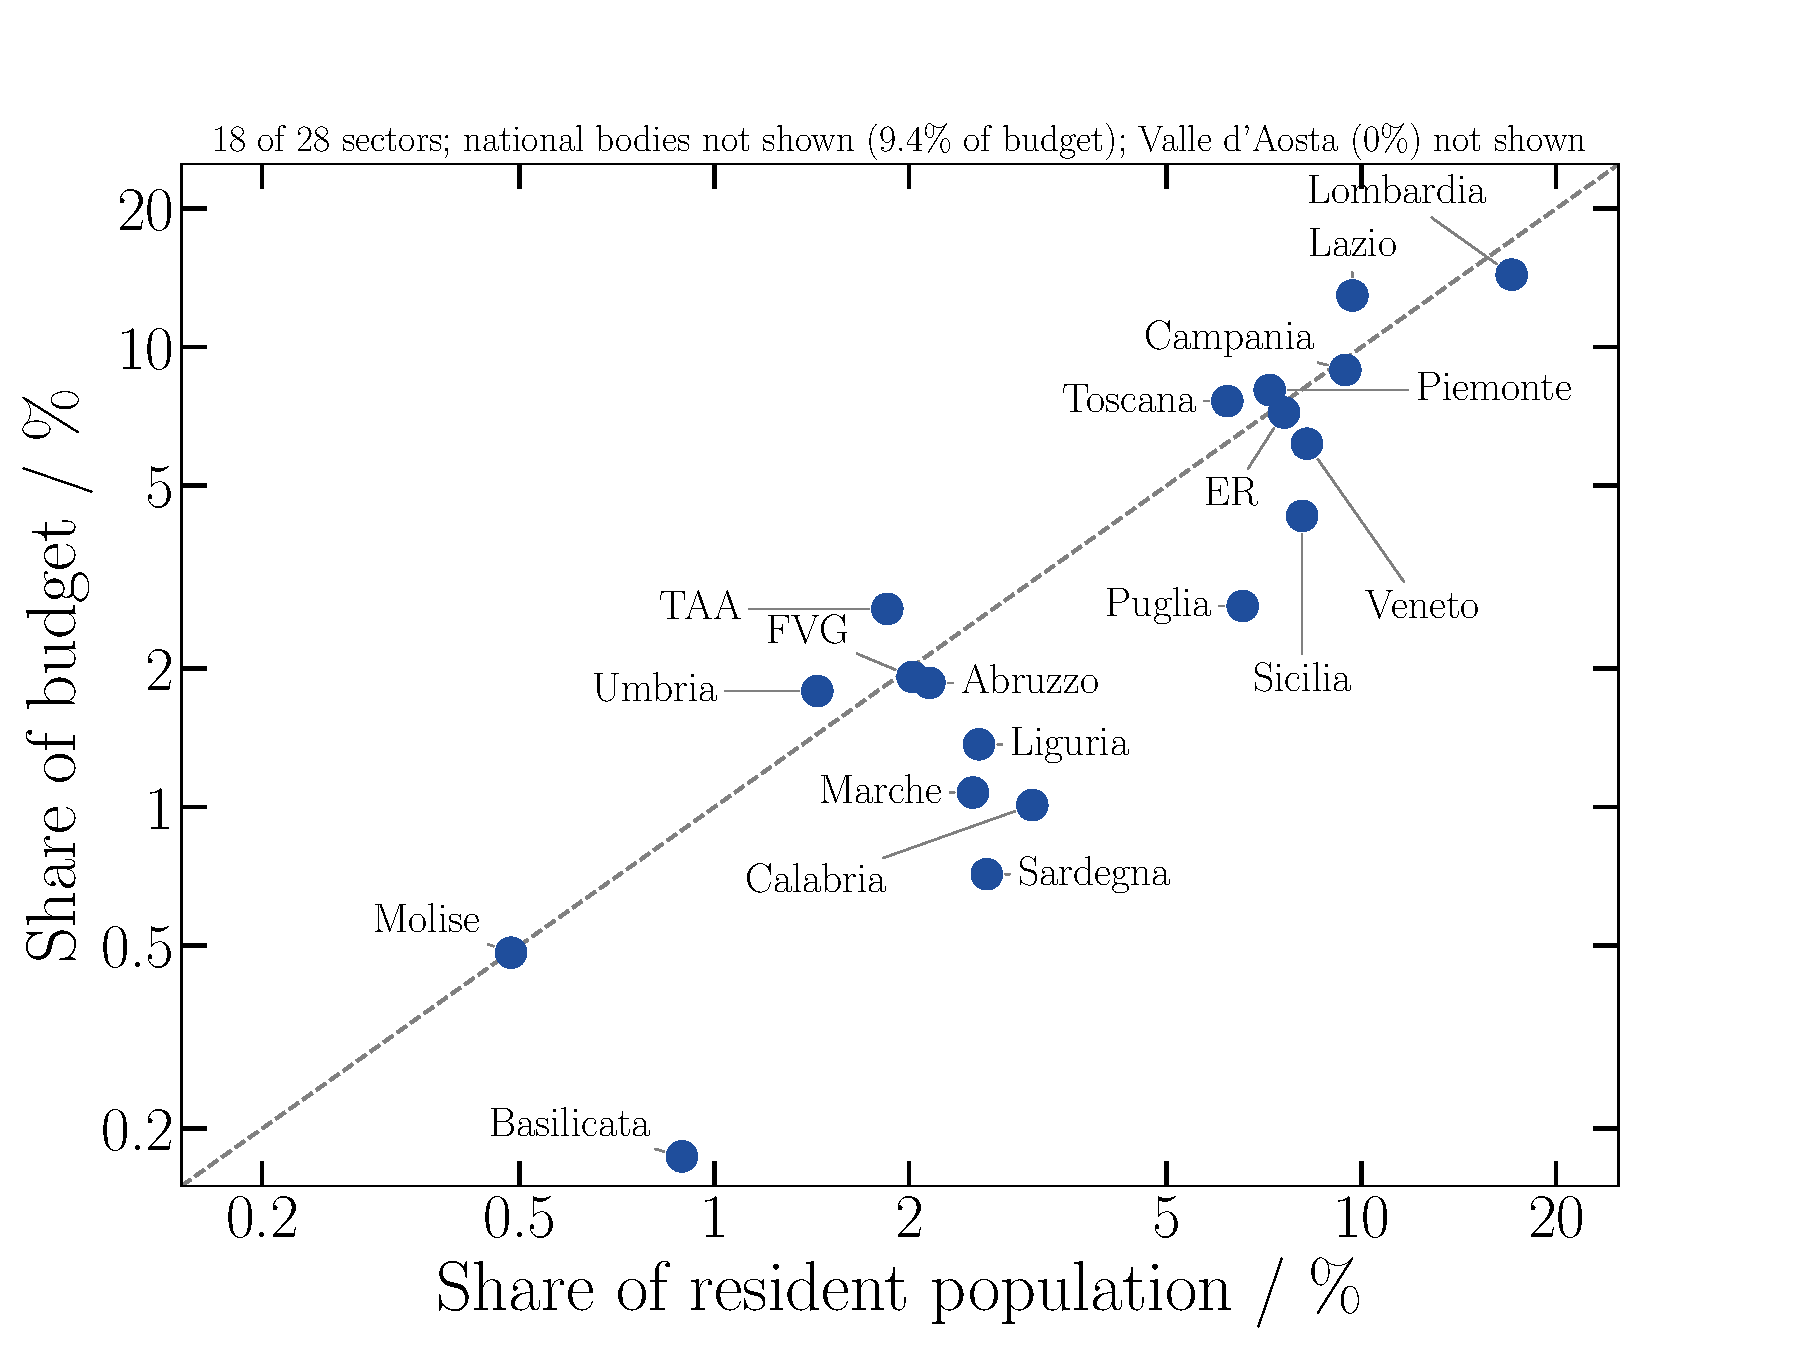
\includegraphics[width=0.75\textwidth]{../prin_out/figures/population_vs_budget.pdf}
\caption{Share of the budget of each region against its share of the resident population (1 January 2026); logarithmic axes, the dashed line marks equal shares. ER: Emilia-Romagna; FVG: Friuli-Venezia Giulia; TAA: Trentino-Alto Adige.}
\end{figure}
\begin{figure}[H]
\centering
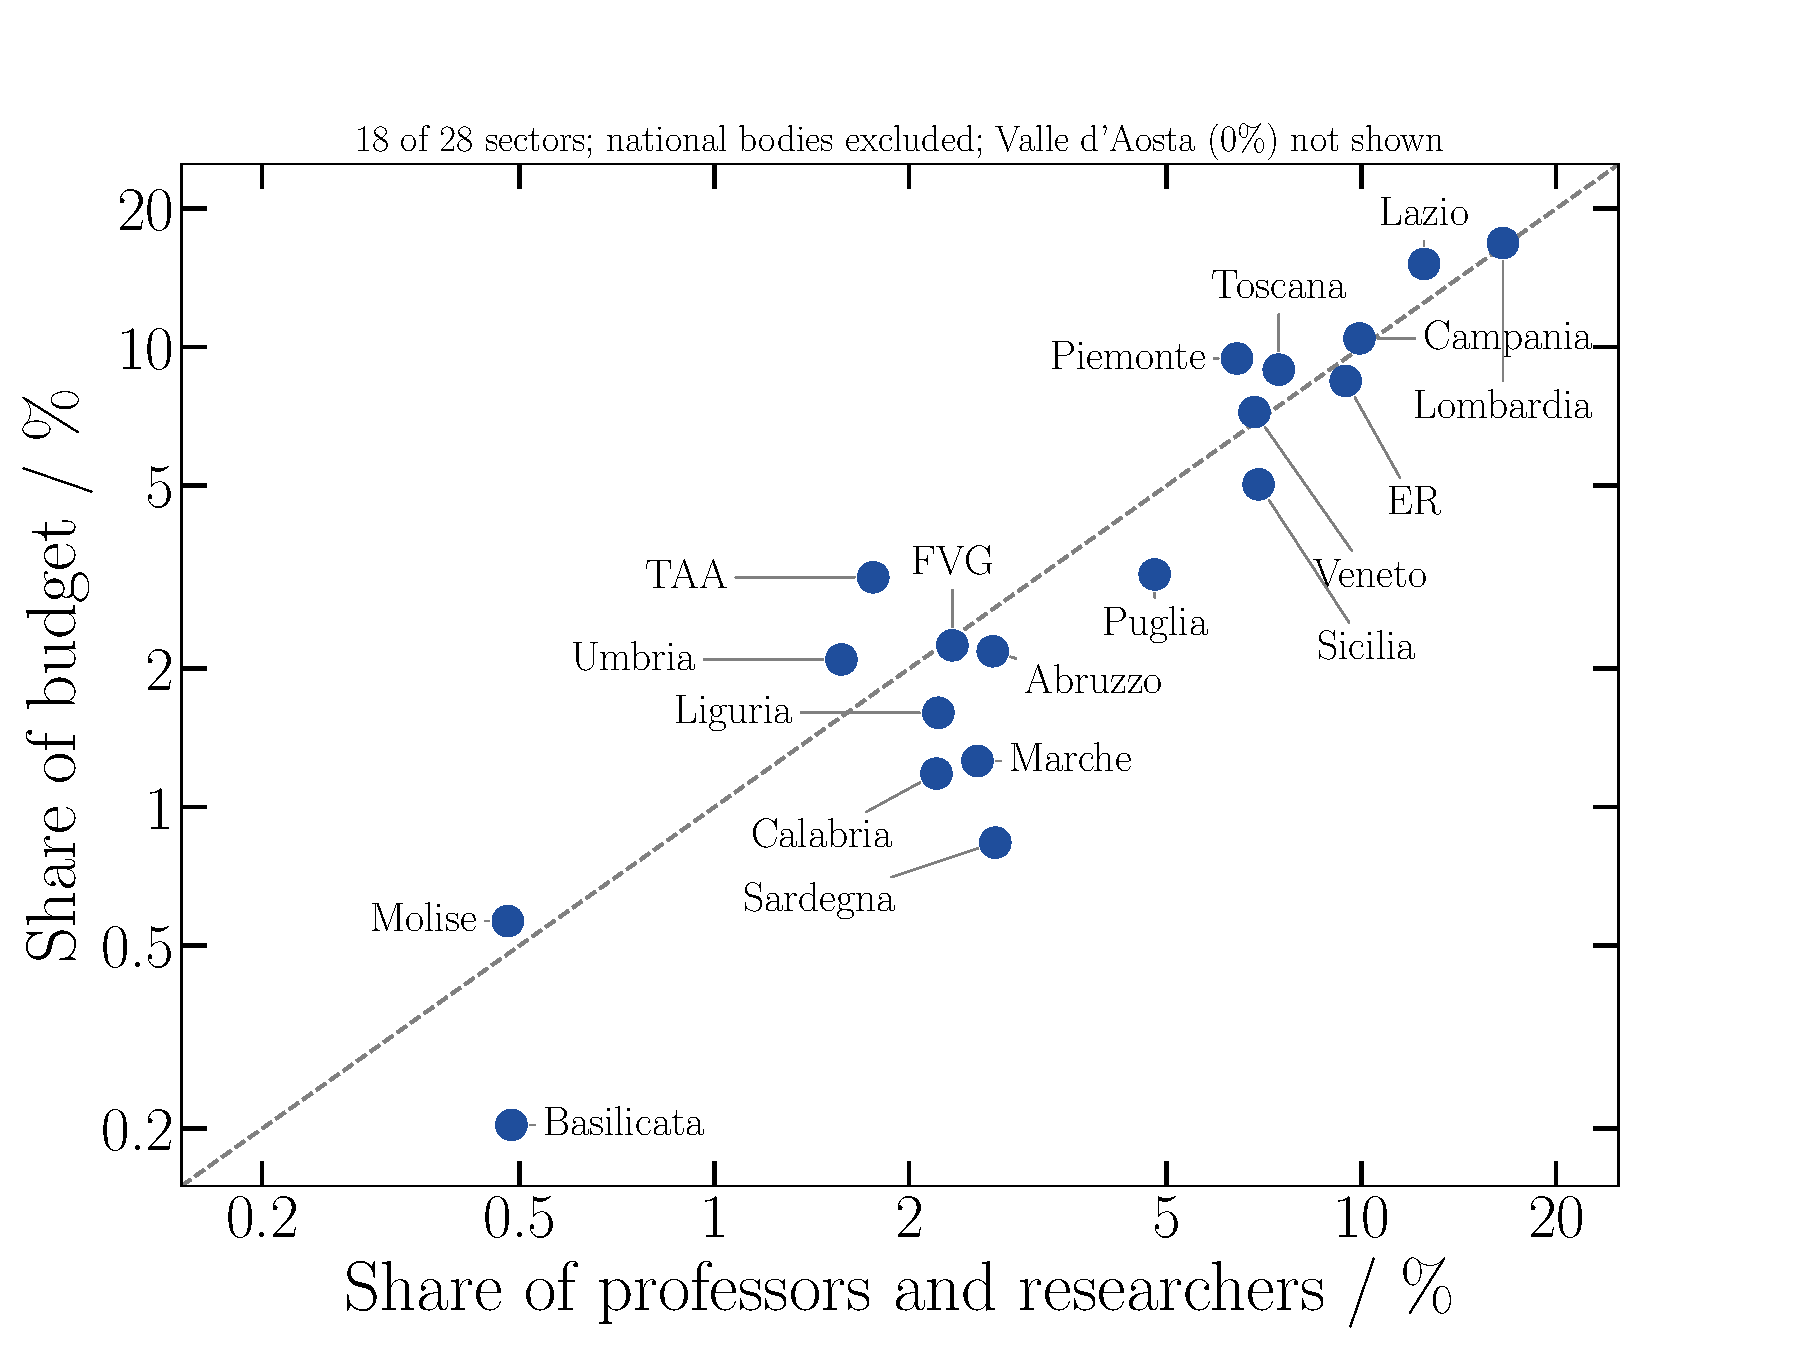
\includegraphics[width=0.75\textwidth]{../prin_out/figures/staff_vs_budget.pdf}
\caption{As above, against the share of professors and researchers of the universities of the region (2024).}
\end{figure}

\subsection{Institution fact sheet: Siena}
\textbf{Purpose.} To collect the figures of one institution and compare them with the other institutions of the same type.

\textbf{Result.} Siena received 1.98~M~EUR (1.21\% of the budget) in 8 projects, 5 as coordinator and 3 as partner, in 7 sectors; it ranks 26 of 84 institutions and 24 of 58 within its type.

\begin{table}[H]
\centering
\begin{tabular}{llr}
\toprule
Siena & Value & Median, public univ. \\
\midrule
Funding & 1.98~M~EUR, 1.21\% of the budget & 0.89\% \\
Rank & 26 of 84; 24 of 58 in its type &  \\
Funded projects & 8 & 7 \\
Sectors with a funded unit & 7 of 18 & 6 \\
Money received as PI & 74\% & 19\% \\
\bottomrule
\end{tabular}
\end{table}
\begin{table}[H]
\centering
\footnotesize
\begin{tabular}{llrp{5.2cm}p{2.2cm}p{4cm}}
\toprule
Sector & Role & k EUR & Project & Coordinator & Other institutions \\
\midrule
LS4 & RU & 164 & Addressing the immunometabolic landscape fueling... & Milano Statale & Bari Aldo Moro, Cattolica, Magna Graecia, Vanvitelli \\
LS7 & PI & 378 & Integrative Tumor and cfDNA Methylation Analysis to Predict... & this institution & Bari Aldo Moro, Federico II, Torino \\
LS7 & PI & 255 & ENDOCARE: CB2 receptor targeting in endometriosis —... & this institution & Chieti-Pescara, L'Aquila, Parma, UniCamillus \\
PE5 & RU & 173 & TWIST — ToWard chiral light from Inverted Singlet-Triplet... & Padova & Basilicata, Bolzano, Brescia, Torino \\
PE7 & RU & 175 & Modular Surfaces with AI-driven Conversion for Integrated... & Firenze & CNR, Catania, Perugia, Politecnico di Milano \\
SH4 & PI & 249 & Accent Representation, Ideologies, and Attitudes (ARIA) & this institution & CNR, Salerno, Sapienza, Tor Vergata \\
SH5 & PI & 387 & DAPHNE – Digital Archive of Petrarchan Heritage and... & this institution & Cattolica, Ferrara, Pegaso, Perugia \\
SH6 & PI & 197 & AFTER: Afterlives of fascism in everyday spaces & this institution & L'Aquila, Padova, Torino, Trento \\
\bottomrule
\end{tabular}
\end{table}
\begin{figure}[H]
\centering
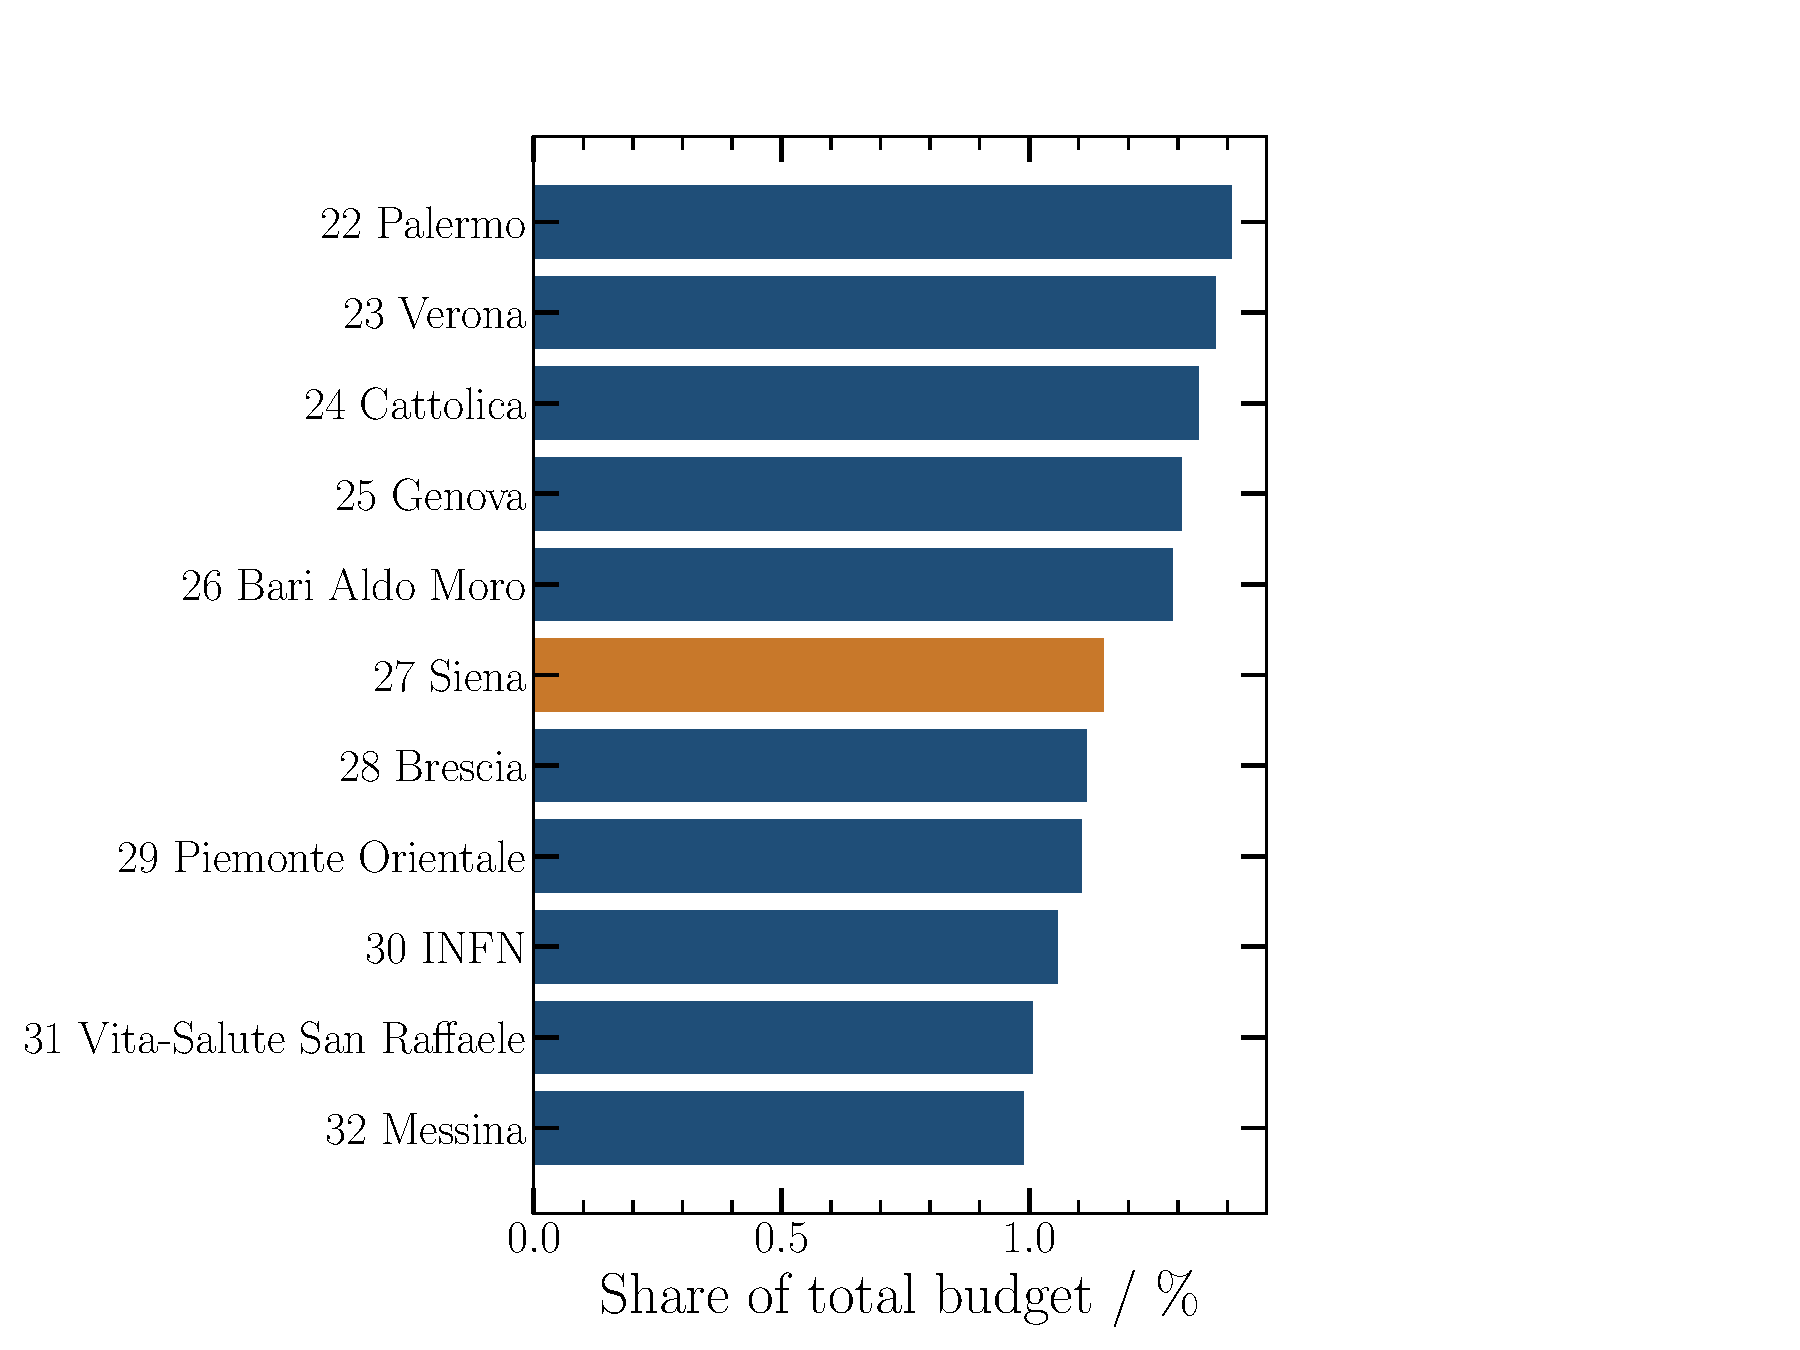
\includegraphics[width=0.65\textwidth]{../prin_out/figures/highlight_neighbours.pdf}
\caption{Share of the total budget of Siena and of the institutions ranked just above and below it.}
\end{figure}
\begin{figure}[H]
\centering
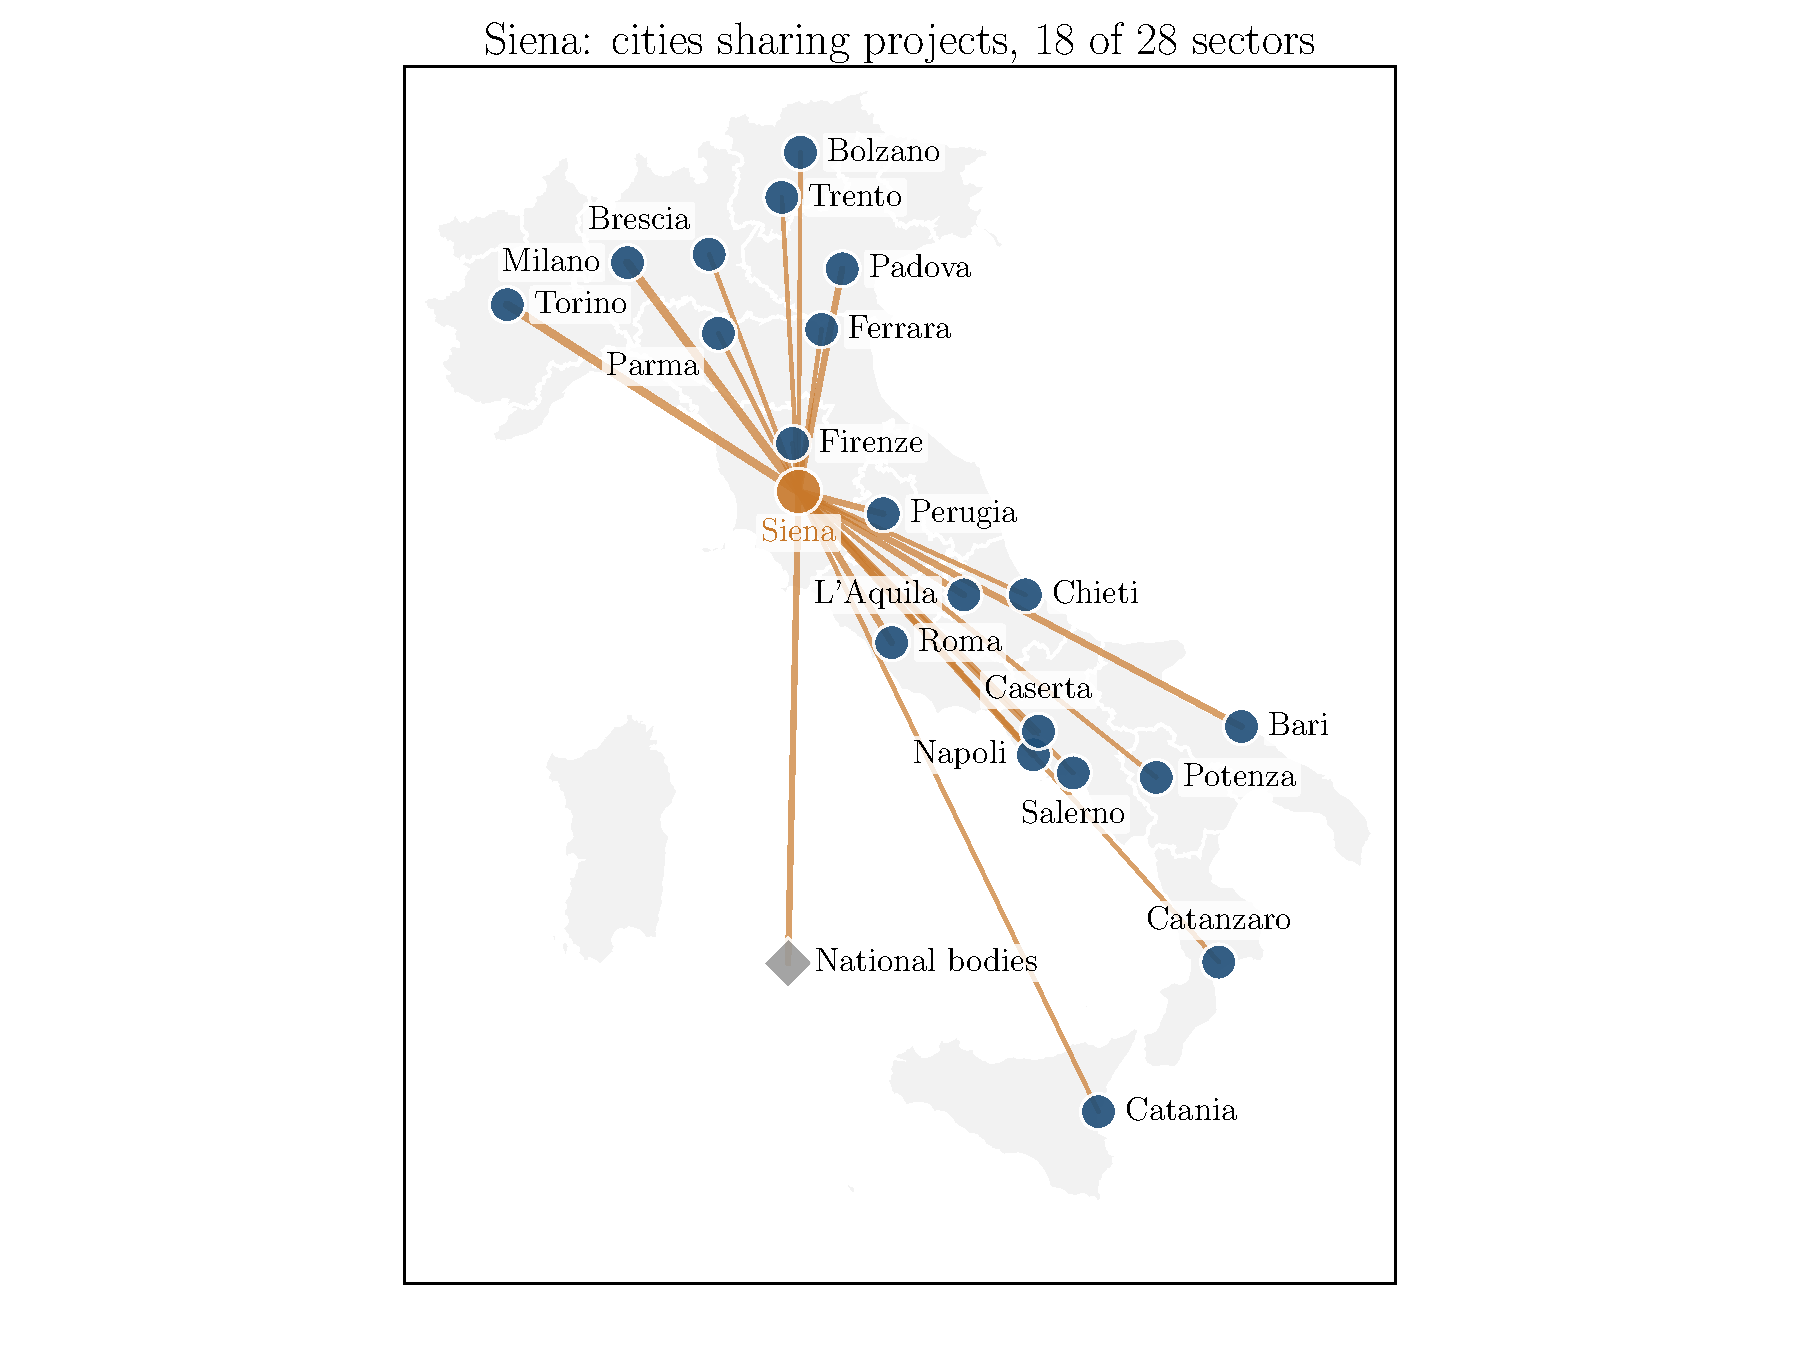
\includegraphics[width=0.75\textwidth]{../prin_out/figures/highlight_map.pdf}
\caption{Cities sharing funded projects with Siena (line width proportional to the number of projects).}
\end{figure}

\appendix
\section{Decrees}
\begin{table}[H]
\centering
\begin{tabular}{llll}
\toprule
Sector & Decree n. & Date & MUR page \\
\midrule
LS2 & 37 & 06/10/2026 & \href{https://www.mur.gov.it/it/atti-e-normativa/bando-prin-2026-ddg-6-ottobre-2026-n-37-macrosettore-ls-settore-ls2-approvazione}{page} \\
LS3 & 38 & 06/10/2026 & \href{https://www.mur.gov.it/it/atti-e-normativa/bando-prin-2026-ddg-6-ottobre-2026-n-38-macrosettore-ls-settore-ls3-approvazione}{page} \\
LS4 & 42 & 06/10/2026 & \href{https://www.mur.gov.it/it/atti-e-normativa/bando-prin-2026-ddg-6-ottobre-2026-n-42-macrosettore-ls-settore-ls4-approvazione}{page} \\
LS7 & 39 & 06/10/2026 & \href{https://www.mur.gov.it/it/atti-e-normativa/bando-prin-2026-ddg-6-ottobre-2026-n-39-macrosettore-ls-settore-ls7-approvazione}{page} \\
PE1 & 29 & 05/10/2026 & \href{https://www.mur.gov.it/it/atti-e-normativa/decreto-direttoriale-n29-del-05-10-2026}{page} \\
PE2 & 30 & 05/10/2026 & \href{https://www.mur.gov.it/it/atti-e-normativa/decreto-direttoriale-n-30-del-05-10-2026}{page} \\
PE3 & 31 & 05/10/2026 & \href{https://www.mur.gov.it/it/atti-e-normativa/decreto-direttoriale-n31-del-05-10-2026}{page} \\
PE5 & 47 & 08/10/2026 & \href{https://www.mur.gov.it/it/atti-e-normativa/decreto-direttoriale-n47-del-08-10-2026}{page} \\
PE6 & 48 & 08/10/2026 & \href{https://www.mur.gov.it/it/atti-e-normativa/decreto-direttoriale-n-48-del-08-10-2026}{page} \\
PE7 & 45 & 06/10/2026 & \href{https://www.mur.gov.it/it/atti-e-normativa/bando-prin-2026-ddg-6-ottobre-2026-n-45-macrosettore-pe-settore-pe7-approvazione}{page} \\
PE8 & 33 & 05/10/2026 & \href{https://www.mur.gov.it/it/atti-e-normativa/decreto-direttoriale-n33-del-05-10-2026}{page} \\
PE9 & 34 & 05/10/2026 & \href{https://www.mur.gov.it/it/atti-e-normativa/decreto-direttoriale-n34-del-05-10-2026}{page} \\
PE10 & 35 & 05/10/2026 & \href{https://www.mur.gov.it/it/atti-e-normativa/decreto-direttoriale-n35-del-05-10-2026}{page} \\
PE11 & 36 & 05/10/2026 & \href{https://www.mur.gov.it/it/atti-e-normativa/decreto-direttoriale-n36-del-05-10-2026}{page} \\
SH4 & 40 & 06/10/2026 & \href{https://www.mur.gov.it/it/atti-e-normativa/bando-prin-2026-ddg-6-ottobre-2026-n-40-macrosettore-sh-settore-sh4-approvazione}{page} \\
SH5 & 41 & 06/10/2026 & \href{https://www.mur.gov.it/it/atti-e-normativa/bando-prin-2026-ddg-6-ottobre-2026-n-41-macrosettore-sh-settore-sh5-approvazione}{page} \\
SH6 & 44 & 06/10/2026 & \href{https://www.mur.gov.it/it/atti-e-normativa/bando-prin-2026-ddg-6-ottobre-2026-n-44-macrosettore-sh-settore-sh6-approvazione}{page} \\
SH7 & 49 & 09/10/2026 & \href{https://www.mur.gov.it/it/atti-e-normativa/decreto-direttoriale-n-49-del-09-10-2026}{page} \\
\bottomrule
\end{tabular}
\end{table}
\section{Sectors}
\begin{table}[H]
\centering
\footnotesize
\begin{tabular}{lrrrrrrr}
\toprule
Sector & Available & Funded & Funded (\%) & Projects & Ranked & Under-40 pool & Under-40 PIs' projects \\
\midrule
LS2 & 6.53~M~EUR & 5.43~M~EUR & 83.2 & 5 & 8 & 0.91~M~EUR & 1.05~M~EUR \\
LS3 & 5.66~M~EUR & 4.67~M~EUR & 82.5 & 4 & 7 & 0.78~M~EUR & 0.00~M~EUR \\
LS4 & 12.94~M~EUR & 12.09~M~EUR & 93.4 & 12 & 16 & 1.85~M~EUR & 2.05~M~EUR \\
LS7 & 17.88~M~EUR & 17.88~M~EUR & 100.0 & 17 & 28 & 3.06~M~EUR & 5.17~M~EUR \\
PE1 & 5.52~M~EUR & 5.52~M~EUR & 100.0 & 5 & 8 & 1.04~M~EUR & 2.16~M~EUR \\
PE2 & 7.32~M~EUR & 6.99~M~EUR & 95.6 & 6 & 12 & 1.20~M~EUR & 2.40~M~EUR \\
PE3 & 5.98~M~EUR & 5.14~M~EUR & 86.0 & 5 & 8 & 0.84~M~EUR & 0.00~M~EUR \\
PE5 & 8.22~M~EUR & 8.22~M~EUR & 100.0 & 8 & 12 & 1.03~M~EUR & 1.03~M~EUR \\
PE6 & 7.42~M~EUR & 6.95~M~EUR & 93.5 & 6 & 11 & 1.33~M~EUR & 2.40~M~EUR \\
PE7 & 11.79~M~EUR & 11.45~M~EUR & 97.1 & 11 & 18 & 1.54~M~EUR & 1.20~M~EUR \\
PE8 & 16.69~M~EUR & 16.46~M~EUR & 98.6 & 14 & 22 & 2.57~M~EUR & 3.48~M~EUR \\
PE9 & 4.97~M~EUR & 4.29~M~EUR & 86.4 & 4 & 8 & 0.68~M~EUR & 1.06~M~EUR \\
PE10 & 9.41~M~EUR & 9.24~M~EUR & 98.2 & 9 & 14 & 1.20~M~EUR & 3.08~M~EUR \\
PE11 & 6.49~M~EUR & 6.49~M~EUR & 100.0 & 6 & 10 & 1.05~M~EUR & 2.17~M~EUR \\
SH4 & 9.62~M~EUR & 8.12~M~EUR & 84.4 & 8 & 16 & 1.50~M~EUR & 1.02~M~EUR \\
SH5 & 10.50~M~EUR & 10.22~M~EUR & 97.3 & 9 & 16 & 1.47~M~EUR & 4.50~M~EUR \\
SH6 & 9.37~M~EUR & 9.25~M~EUR & 98.6 & 9 & 14 & 1.16~M~EUR & 5.14~M~EUR \\
SH7 & 7.70~M~EUR & 7.00~M~EUR & 91.0 & 6 & 7 & 1.11~M~EUR & 2.21~M~EUR \\
\bottomrule
\end{tabular}
\end{table}
\section{Regions}
\begin{table}[H]
\centering
\footnotesize
\begin{tabular}{lrrrrr}
\toprule
Region & Share (\%) & Projects & PI units & RU units & As PI (\%) \\
\midrule
Piemonte & 8.06 & 54 & 14 & 43 & 31 \\
Valle d'Aosta & 0.00 & 0 & 0 & 0 &  \\
Liguria & 1.37 & 11 & 0 & 11 & 0 \\
Lombardia & 14.36 & 81 & 27 & 82 & 32 \\
Trentino-Alto Adige & 2.70 & 21 & 5 & 16 & 30 \\
Veneto & 6.16 & 45 & 15 & 31 & 40 \\
Friuli-Venezia Giulia & 1.92 & 14 & 5 & 10 & 38 \\
Emilia-Romagna & 7.20 & 48 & 8 & 47 & 19 \\
Marche & 1.08 & 9 & 2 & 7 & 25 \\
Toscana & 7.63 & 52 & 14 & 42 & 30 \\
Umbria & 1.79 & 13 & 1 & 13 & 8 \\
Lazio & 12.94 & 78 & 14 & 94 & 17 \\
Campania & 8.91 & 49 & 15 & 54 & 28 \\
Abruzzo & 1.86 & 14 & 4 & 11 & 32 \\
Molise & 0.48 & 4 & 0 & 4 & 0 \\
Puglia & 2.74 & 21 & 2 & 21 & 9 \\
Basilicata & 0.17 & 2 & 0 & 2 & 0 \\
Calabria & 1.01 & 10 & 0 & 10 & 0 \\
Sicilia & 4.29 & 30 & 7 & 27 & 25 \\
Sardegna & 0.71 & 6 & 2 & 4 & 47 \\
National research bodies & 9.36 & 58 & 9 & 53 & 22 \\
\bottomrule
\end{tabular}
\end{table}
\section{All institutions}
Institutions with at least one funded unit, by funding (the region of each is in the institution table of the analysis output); share of the total budget, MUR contribution, projects, units as coordinator (PI) and partner (RU), sectors with a funded unit.

{\footnotesize\setlength{\tabcolsep}{2.5pt}
\begin{longtable}{rlllrrrrrr}
\toprule
Rank & Institution & Type & City & Share (\%) & k EUR & Proj. & PI & RU & Sect. \\
\midrule
\endhead
1 & CNR & National bodies & Roma & 7.20 & 11810 & 49 & 8 & 41 & 15 \\
2 & Sapienza & Public univ. & Roma & 6.18 & 10131 & 50 & 7 & 43 & 15 \\
3 & Padova & Public univ. & Padova & 4.59 & 7521 & 35 & 11 & 24 & 16 \\
4 & Torino & Public univ. & Torino & 4.23 & 6943 & 31 & 6 & 25 & 15 \\
5 & Bologna & Public univ. & Bologna & 3.76 & 6161 & 27 & 5 & 22 & 14 \\
6 & Federico II & Public univ. & Napoli & 3.62 & 5933 & 29 & 7 & 22 & 11 \\
7 & Firenze & Public univ. & Firenze & 3.23 & 5291 & 24 & 5 & 19 & 11 \\
8 & Milano Statale & Public univ. & Milano & 3.20 & 5246 & 25 & 9 & 16 & 13 \\
9 & Politecnico di Milano & Public univ. & Milano & 2.49 & 4088 & 19 & 2 & 17 & 8 \\
10 & Trento & Public univ. & Trento & 2.49 & 4078 & 19 & 5 & 14 & 11 \\
11 & Politecnico di Torino & Public univ. & Torino & 2.40 & 3941 & 16 & 7 & 9 & 6 \\
12 & Pisa & Public univ. & Pisa & 2.37 & 3882 & 18 & 3 & 15 & 12 \\
13 & Milano-Bicocca & Public univ. & Milano & 2.29 & 3762 & 16 & 8 & 8 & 9 \\
14 & Salerno & Public univ. & Salerno & 2.16 & 3535 & 15 & 5 & 10 & 7 \\
15 & Tor Vergata & Public univ. & Roma & 2.09 & 3425 & 18 & 0 & 18 & 10 \\
16 & Parma & Public univ. & Parma & 1.90 & 3115 & 16 & 1 & 15 & 13 \\
17 & Catania & Public univ. & Catania & 1.78 & 2925 & 15 & 3 & 12 & 9 \\
18 & Vanvitelli & Public univ. & Caserta & 1.72 & 2823 & 13 & 2 & 11 & 4 \\
19 & Roma Tre & Public univ. & Roma & 1.68 & 2753 & 13 & 3 & 10 & 8 \\
20 & Perugia & Public univ. & Perugia & 1.64 & 2686 & 13 & 0 & 13 & 7 \\
21 & Palermo & Public univ. & Palermo & 1.48 & 2419 & 11 & 3 & 8 & 8 \\
22 & Genova & Public univ. & Genova & 1.37 & 2245 & 11 & 0 & 11 & 10 \\
23 & Cattolica & Private univ. & Milano & 1.29 & 2112 & 10 & 1 & 9 & 5 \\
24 & Pavia & Public univ. & Pavia & 1.28 & 2095 & 10 & 2 & 8 & 7 \\
25 & Bari Aldo Moro & Public univ. & Bari & 1.24 & 2031 & 10 & 0 & 10 & 6 \\
26 & Siena & Public univ. & Siena & 1.21 & 1978 & 8 & 5 & 3 & 7 \\
27 & Piemonte Orientale & Public univ. & Vercelli & 1.16 & 1899 & 8 & 1 & 7 & 8 \\
28 & Verona & Public univ. & Verona & 1.14 & 1864 & 7 & 4 & 3 & 6 \\
29 & INFN & National bodies & Roma & 1.11 & 1817 & 6 & 0 & 6 & 4 \\
30 & Messina & Public univ. & Messina & 1.04 & 1699 & 8 & 1 & 7 & 6 \\
31 & Modena e Reggio Emilia & Public univ. & Modena & 0.92 & 1505 & 7 & 1 & 6 & 6 \\
32 & Vita-Salute San Raffaele & Private univ. & Milano & 0.90 & 1480 & 6 & 2 & 4 & 5 \\
33 & Trieste & Public univ. & Trieste & 0.90 & 1468 & 7 & 3 & 4 & 7 \\
34 & Brescia & Public univ. & Brescia & 0.89 & 1466 & 8 & 0 & 8 & 6 \\
35 & L'Aquila & Public univ. & L'Aquila & 0.80 & 1308 & 7 & 1 & 6 & 6 \\
36 & INAF & National bodies & Roma & 0.78 & 1272 & 4 & 1 & 3 & 1 \\
37 & Insubria & Public univ. & Varese & 0.76 & 1240 & 6 & 1 & 5 & 4 \\
38 & Parthenope & Public univ. & Napoli & 0.74 & 1210 & 6 & 1 & 5 & 5 \\
39 & Cassino & Public univ. & Cassino & 0.66 & 1081 & 6 & 2 & 4 & 2 \\
40 & Calabria & Public univ. & Rende & 0.65 & 1068 & 6 & 0 & 6 & 4 \\
41 & SISSA & Advanced schools & Trieste & 0.64 & 1049 & 5 & 2 & 3 & 3 \\
42 & Ferrara & Public univ. & Ferrara & 0.63 & 1033 & 5 & 1 & 4 & 5 \\
43 & GSSI & Advanced schools & L'Aquila & 0.62 & 1010 & 4 & 3 & 1 & 3 \\
44 & Cagliari & Public univ. & Cagliari & 0.60 & 978 & 5 & 2 & 3 & 4 \\
45 & Foggia & Public univ. & Foggia & 0.52 & 849 & 5 & 0 & 5 & 3 \\
46 & Unicusano & Telematic univ. & Roma & 0.49 & 799 & 4 & 0 & 4 & 3 \\
47 & Link Campus University & Private univ. & Roma & 0.49 & 798 & 5 & 0 & 5 & 3 \\
48 & Molise & Public univ. & Campobasso & 0.48 & 791 & 4 & 0 & 4 & 3 \\
49 & IUSS Pavia & Advanced schools & Pavia & 0.48 & 788 & 2 & 2 & 0 & 2 \\
50 & Camerino & Public univ. & Camerino & 0.47 & 764 & 4 & 1 & 3 & 3 \\
51 & Salento & Public univ. & Lecce & 0.44 & 724 & 4 & 1 & 3 & 4 \\
52 & IMT Lucca & Advanced schools & Lucca & 0.43 & 710 & 3 & 0 & 3 & 1 \\
53 & Tuscia & Public univ. & Viterbo & 0.43 & 706 & 3 & 2 & 1 & 3 \\
54 & Campus Bio-Medico & Private univ. & Roma & 0.43 & 698 & 4 & 0 & 4 & 3 \\
55 & Politecnico di Bari & Public univ. & Bari & 0.40 & 658 & 3 & 0 & 3 & 2 \\
56 & Chieti-Pescara & Public univ. & Chieti & 0.37 & 610 & 3 & 0 & 3 & 3 \\
57 & Magna Graecia & Public univ. & Catanzaro & 0.36 & 588 & 4 & 0 & 4 & 3 \\
58 & e-Campus & Telematic univ. & Novedrate & 0.36 & 587 & 3 & 0 & 3 & 3 \\
59 & Ca' Foscari & Public univ. & Venezia & 0.31 & 516 & 3 & 0 & 3 & 2 \\
60 & Humanitas University & Private univ. & Pieve Emanuele & 0.31 & 507 & 3 & 0 & 3 & 1 \\
61 & Politecnica delle Marche & Public univ. & Ancona & 0.30 & 500 & 2 & 1 & 1 & 2 \\
62 & INGV & National bodies & Roma & 0.28 & 453 & 3 & 0 & 3 & 1 \\
63 & Pegaso & Telematic univ. & Napoli & 0.27 & 450 & 3 & 0 & 3 & 2 \\
64 & INRiM & Research bodies & Torino & 0.27 & 438 & 2 & 0 & 2 & 2 \\
65 & Sant'Anna & Advanced schools & Pisa & 0.26 & 434 & 2 & 0 & 2 & 2 \\
66 & OGS & Research bodies & Trieste & 0.24 & 388 & 2 & 0 & 2 & 1 \\
67 & Urbino & Public univ. & Urbino & 0.22 & 360 & 2 & 0 & 2 & 2 \\
68 & Bolzano & Public univ. & Bolzano & 0.21 & 344 & 2 & 0 & 2 & 2 \\
69 & UniCamillus & Private univ. & Roma & 0.20 & 336 & 2 & 0 & 2 & 1 \\
70 & San Raffaele Roma & Telematic univ. & Roma & 0.20 & 335 & 2 & 0 & 2 & 2 \\
71 & Basilicata & Public univ. & Potenza & 0.17 & 285 & 2 & 0 & 2 & 2 \\
72 & L'Orientale & Public univ. & Napoli & 0.16 & 257 & 1 & 0 & 1 & 1 \\
73 & Scuola Superiore Meridionale & Advanced schools & Napoli & 0.15 & 250 & 1 & 0 & 1 & 1 \\
74 & Stranieri di Perugia & Public univ. & Perugia & 0.15 & 245 & 1 & 1 & 0 & 1 \\
75 & Udine & Public univ. & Udine & 0.15 & 241 & 1 & 0 & 1 & 1 \\
76 & LUM & Private univ. & Casamassima & 0.14 & 224 & 1 & 1 & 0 & 1 \\
77 & Normale & Advanced schools & Pisa & 0.13 & 211 & 1 & 1 & 0 & 1 \\
78 & IUAV & Public univ. & Venezia & 0.12 & 205 & 1 & 0 & 1 & 1 \\
79 & Sassari & Public univ. & Sassari & 0.12 & 194 & 1 & 0 & 1 & 1 \\
80 & IULM & Private univ. & Milano & 0.12 & 189 & 1 & 0 & 1 & 1 \\
81 & Sannio & Public univ. & Benevento & 0.10 & 163 & 1 & 0 & 1 & 1 \\
82 & Accademia Belle Arti Frosinone & AFAM & Frosinone & 0.10 & 162 & 1 & 0 & 1 & 1 \\
83 & Macerata & Public univ. & Macerata & 0.09 & 141 & 1 & 0 & 1 & 1 \\
84 & Teramo & Public univ. & Teramo & 0.08 & 126 & 1 & 0 & 1 & 1 \\
\bottomrule
\end{longtable}
}
\end{document}
